\documentclass[a4paper, 12pt, titlepage, onecolumn]{article}

%--- USEPACKAGES ---
\usepackage[utf8]{inputenc}
\usepackage{natbib}
\usepackage[brazil]{babel}
\usepackage{epsfig}
\usepackage{subfig}
\usepackage{ae}
\usepackage{aecompl}
\usepackage{booktabs}
\usepackage[T1]{fontenc}
\usepackage{graphicx,wrapfig} % para incluir figuras
\usepackage{amsfonts, amssymb,amsthm, amsmath, amscd} % pacote AMS
\usepackage{color, float, bbm, multicol}
\usepackage{verbatim, listings, booktabs}
\usepackage{fancyhdr} % FANCYHEADER
\usepackage{setspace}
\usepackage{times} % bookman,palatino,courier,times FONTES
\usepackage{lineno}
\usepackage{url}

\hoffset = 0pt % 1inch + hoffset (margem vertical esquerda)
\voffset = 0pt % 1inch + voffset (margem horizontal superior)
\oddsidemargin = 0pt % complemento da margem vertical esquerda
\topmargin = 0pt % complemento da margem horizontal superior
\headheight = 10pt % altura do header
\headsep = 0pt % distancia do header ate o texto
\textheight = 700pt % altura do texto
\textwidth = 470pt % largura do texto
\marginparsep = 0pt % distancia do texto ate a
%margin notes (11pt)
\marginparwidth = 0pt % largura da margin notes (54pt)
\paperheight = 297mm % a4
\paperwidth = 210mm % a4

\title{
  \Large{Relatório Final - v 2.0} \\
  \Huge{Evolução Morfológica e Modularidade }}
\author{Diogo Melo \\
        \textbf {Orientador} Gabriel Marroig\\
  \footnotesize{diogro@gmail.com $\cdot$ gmarroig@usp.br} \\
  \footnotesize{Laboratório de Evolução de Mamíferos} \\
  \footnotesize{Departamento de Genética e Biologia Evolutiva} \\
  \footnotesize{Instituto de Biociências $\cdot$ Universidade de São Paulo} \\
  \footnotesize{Caixa Postal 11.461, CEP 05422 $\cdot$ 970, 
    São Paulo $\cdot$ SP, Brasil.} \\
  \footnotesize{Telefone: +55 $\cdot$ 11 $\cdot$ 3091 $\cdot$ 8759} \\
}

\selectlanguage{brazil}

% --- DEFINICOES ---
\newcommand{\barra}{\backslash}
\newcommand{\To}{\longrightarrow}
\newcommand{\abs}[1]{\left\vert#1\right\vert}
\newcommand{\set}[1]{\left\{#1\right\}}
\newcommand{\seq}[1]{\left<#1\right>}
\newcommand{\norma}[1]{\left\Vert#1\right\Vert}
\newcommand{\hr}{\par\noindent\hrulefill\par}

\numberwithin{equation}{section}
\numberwithin{table}{section}
%\numberwithin{figure}{subsection}
\bibliographystyle{evolution}
% --- O DOCUMENTO EM SI ---
\begin{document}
\pagestyle{plain} % fancy,plain,empty,headings
\renewcommand{\headrulewidth}{0.4pt}
\renewcommand{\footrulewidth}{0.4pt}
\pagenumbering{arabic}
\maketitle
\thispagestyle{plain} % sem barras no header na capa (PAGINA 1)
\hrule % linha estetica
\tableofcontents
% \hrule % nova linha estetica
% \newpage

% >>>>>>>>>>>>>>>>>> INICIO DO TEXTO <<<<<<<<<<<<<<<<<<<

\section{Resumo Inicial}
\doublespacing 
O projeto consiste no estudo de modelos computacionais para a evolução
de traços quantitativos sujeitos a variados tipos de pressões seletivas.
A situação de maior interesse é a de manutenção dos padrões de
correlação entre os caracteres e o efeito dessa seleção estabilizadora
e direcional na distribuição de fenótipos da população. Além disso, procuramos
analisar o efeito do tamanho populacional, número de traços sob seleção e
aparecimento de modularidade nas características dos indivíduos. O uso
de simulações numéricas se presta imensamente a esse tipo de estudo, por
possibilitar um conhecimento real sobre a história evolutiva das
populações estudadas.

\section{Resumo Parcial}

No periodo em questão foi abordada a questão de evolução dos padrões de
modularidade em populações sofrendo seleção natural, deriva e mutação.
Dois tipos de modelos computacionais foram implementados e testados na
sua capacidade de reproduzir padrões naturais, principalmente o de
emergencia de padrões de covariação modulares. Exploramos condições para
a emergencia e manutenção modularidade variacional em populações
sujeitas a diferentes tipos de seleção natural, mutação, esquemas de
simulação de traços quantitativos, com variados tamanhos populacionais e
niveis de complexidade.

\section{Introdução}
\linenumbers
\modulolinenumbers[1]

O estudo de traços quantitativos se baseia amplamente na teoria da
genética quantitativa. Essa teoria permite entender a evolução de
caracteres continuos de forma bastante completa. Para isso são
utilizadas de medidas quantitativas de traços morfológicos. A equação
multi-variada de resposta à seleção, $\Delta z = G \beta$, proposta por
\cite{Lande1979} permite ligar a mudança na média de um conjunto de
caracteres ($\Delta z$) à seleção imposta à população ($\beta$) e à sua
matriz de covariação genética aditiva (G). Além disso, esse mesmo
raciocínio pode ser usado para investigar padrões macro-evolutivos de
resposta ao longo de muitas gerações \citep{Lande1983, Marroig2004,
Marroig2005}.  

Porém, nossa habilidade de inferir a resposta evolutiva a muitas
gerações de seleção depende fundamentalmente da constância da matriz G
ao longo de muitas gerações, e a teoria de Lande não explora
detalhadamente a dinâmica da própria matriz G, assumindo implicitamente
nas equações sua constância ao supor que a distribuição das
características na população é sempre gaussiana.  Essa suposição
simplificadora de Lande se baseia em um resultado derivado do modelo
apresentado em \cite{Crow1964}, chamado de modelo do continuo de alelos.
Neste modelo a distribuição de efeitos alélicos sobre um determinado
caráter é contínuo, e em \cite{Kimura1965} foi demonstrada que a
distribuição de equilibrio dos efeito alélicos em uma população sofrendo
mutação, deriva e seleção estabilizadora é gaussiana, com a suposição de
que os efeitos mutacionais são pequenos frente à variação existente na
população. Ou seja, assumindo que os efeitos alélicos sejam efetivamente
gaussianos, a dinâmica da média da população pode ser completamente
descrita apenas pela média e pela matriz de covariação desses efeitos
\citep{Barton1987}. 

Notamos então que uma série de suposições não triviais devem ser feitas
para que esse modelo gaussiano quadrático de Lande seja teoricamente
plausível. Esses problemas foram apresentados ao longo da década de 80
por uma série de artigos, principalmente e pioneiramente por
\citep{Turelli1984, Turelli1985, Turelli1986, Barton1987}. Talvez a
questão mais importante seja a suposição de que os alelos tenham
distribuição contínua poposta por \cite{Crow1964}. Para que isso seja
realista a taxa de mutação por locus deve ser suficientemente alta para
manter a distribuição de alelos por locus gaussiana frente à deriva e
seleção estabilizadora, que removem variabilidade \citep{Falconer1996}.
Além disso podemos nos perguntar se mutações novas realmente tem efeitos
pequenos em relação a variância original da população nas direções
morfológicas afetadas, ou se novas mutações introduzem variabilidade
maior que originalmente presente na população. O modelo proposto por
\cite{Turelli1984} utiliza então taxas de mutação baixas e efeitos
mutacionais altos, mas ainda mantendo o espaço de alelos contínuo.
Nessas condições, a matriz G não seria constante ao longo do tempo e
fatores de correção deveriam ser acrescidos à equação de resposta de
Lande para descrições macro-evolutivas. Esses fatores dependem do desvio
por geração da matriz G em relação à matriz G média no periodo de
seleção \citep{Jones2003}. A estimativa desse ``efeito Turelli'' é
difícil de ser realizada praticamente.  

Em \cite{Barton1987}, os autores, interessados no problema dá dinâmica
das variâncias de forma geral, apresentam um formalismo relativamente
completo para lidar com o problema da evolução de todos os momentos da
distribuição fenotípica de um traço quantitativo, abordando tanto a
aproximação gaussiana quanto a aproximação de alelos raros, proposta por
\cite{Turelli1984}. O procedimento seguido pelos autores é escrever a
dinâmica de mudança de todos o momentos da distribuição de efeitos
alélicos da população sujeita a uma pressão de seleção na forma de uma
subida de gradiente imposta por uma superfície de seleção arbritária
(mas com todas as derivadas parciais bem definidas no espaço dos
momentos) \citep{Arnold2001a}. Isso permite abarcar o formalismo de
Lande, tomando apenas os dois primeiros momentos (média e variância),
supondo o segundo momento fixo e desprezando os momentos mais altos; ou
incluir mudanças até uma certa ordem e obter os resultados de Turelli. 

% Continuar Turelli Barton?

Dada a complexidade do problema da dinâmica das variâncias em um caso
multi-variado, o estudo da estabilidade da matriz G e suas consequências
para o estudo da evolução de caracteres quantitativos se tornou um
problema eminentemente experimental, sejam esses experimentos conduzidos
de forma restrospectiva, amostrando a diversidade dos seres vivos, seja
em experimentos manipulativos feitos com colônias de animais em cativeiro ou,
como é o caso do presente trabalho, por via de simulações
computacionais. Vamos agora revisar as principais abordagens computacionais e empíricas 
.

A sequência de artigos \cite{Jones2003, Jones2004, Jones2007} foi
pioneira nos estudos computacionais de estabilidade da matriz G num
contexto multivariado moderno, abordando o tema da evolução de dois
caracteres correlacionados em diferentes situações. O estilo de
simulação apresentado em \cite{Jones2003} e utilizado em todos os
artigos subsequentes serviu de ponto de partida para nossas simulações e
será descrito em detalhes nas próximas seções.


O problema mais simples, abordado em \cite{Jones2003}, consiste no estudo
de estabilidade da matriz G associada a dois caracteres quantitativos
com interações pleiotrópicas fixas em uma população finita sofrendo
mutação, deriva e seleção estabilizadora gaussiana. Os principais
parâmetros que influem na estabilidade da matriz G nessas simulações são
o padrão de mutação pleitotrópico e a superfície de seleção. Ambos são
descritos por matrizes de covariância. Os valores na diagonal dessas
matrizes representam a intensidade das mutações e a intensidade da
seleção estabilizadora em cada traço separadamente. Como o problema é
bidimensional, essas matrizes tem apenas um valor fora da diagonal. Esse
valor é apresentado como uma correlação de mutação no
caso da matriz mutacional ($r_\mu$) e uma correlação de seleção na matriz
que descreve a superfície de adptidão ou {\it fitness} ($r_\omega$). O valor de $r_\mu$
define o quão correlacionados serão os valores das mutações que afetam
ambos os traços. Quanto mais alto, mais correlacionados eles serão, com
sua magnitude dada pelos valores diagonais da matriz de mutação. Já o
valor de $r_\omega$ define o quão forte é a seleção estabilizadora no
sentido de manter os dois traços correlacionados. Nas condições das simulações, o
fator mais importante para a estabilidade da matriz G foi a existência de
mutações correlacionadas. Quando $r_\mu$ e $r_\omega$ são similares, a
matriz tende a ser bastante estável. Além disso, tamanhos populacionais
grandes também contribuem para a estabilidade da matriz.
Um resultado interessante é que existem tipos diferentes de estabilidade
para matrizes de covariância. Por exemplo: uma matriz pode manter seus
auto-valores estáveis, não sofrendo alterações na quantidade de
variância genética disponível, mas ter auto-vetores variáveis, alterando
assim em qual direção do morfo-espaço a variabilidade populacional está
disponível para responder a seleção. Os autores ressaltam que matrizes com um auto-valor
dominante tendem a ser mais estáveis. Ou seja, correlação alta entre os
dois traços leva à estabilidade da matriz G. Isso pode ser interpretado como um
primeiro indício para a importância da modularidade (veja abaixo), apesar de ser
difícil definir modularidade de maneira convincente com apenas dois
caracteres. Em resumo, esse artigo mostra que é possível observarmos
matrizes estáveis em condições plausivelmente naturais, e dá o primeiro
passo para a quantificação dessas condições.

O próximo passo foi a inclusão de seleção direcional em
\cite{Jones2004}. O estilo de simulação é basicamente idêntico ao artigo
anterior, mas agora a posição do pico adaptativo gaussiano é variado,
alterando assim a média da população e criando uma seleção direcional.
Além de permitir abordar a questão da estabilidade sob novas condições,
essa nova simulação permite também explorar a reconstrução da seleção
direcional via equação de \cite{Lande1979} e quantificar o efeito de
Turelli devido a flutuações na matriz G. Para entender o efeito Turelli,
vamos explorar como a extensão da equação de Lande deve ser feita para
abarcar a mudança evolutiva ao longo de várias gerações. Começamos com a
equação de resposta à seleção nas médias dos traços ($\overline {z}$)
para uma única geração de uma população sujeita ao gradiente de seleção
$\beta_t$:

\begin{equation}
\Delta \overline {z} = \overline {z}_{t+1}-\overline {z}_{t}=G\beta_t
\end{equation}

Com essa equação, e de posse das médias antes e depois da seleção e da
matriz G dessa população, podemos estimar o valor de $\beta_t$. Além
disso, podemos pensar em definir um gradiente médio $\beta_T$  ao longo
de várias gerações de seleção \citep{Lande1979}, como:

\begin{equation}
\beta_{T}\equiv \sum _{t=0}^{T-1} \beta_t =  \overline {G}^{-1}\Delta \overline {z}_T 
\end{equation}

ou seja, a soma dos gradientes individuais, onde $\overline {G}$
representa a matriz G média e $\Delta \overline {z}_T$ a mudança global
na média dos traços. \cite{Turelli1988} mostrou que essa equação se
torna incorreta caso a flutuação da matriz G em torno da média seja
grande entre uma geração e outra. Isso fica claro expandindo essa equação
de forma a mostrar os termos de flutuação:
\begin{equation}
   \beta_T = \overline {G}^{-1} \left[ \Delta \overline {z}_T - \sum_{t=0}^{T-1} (G_t - \overline {G}) \beta_t\right]
\end{equation}

Se o termo de Turelli (  $\sum_{t=0}^{T-1} (G_t - \overline {G})
\beta_t$ ) for grande, a estimativa de $\beta_T$ será precária. É
necessário então avaliar se a estabilidade da matriz G é suficiente para
manter esse termo pequeno pequeno o bastante para possibilitar a
estimativa de gradientes de seleção realistas. Para isso, foram
realizadas simulações com 3 tipos de movimentos do pico adaptativo: ao
longo da direção de aumento de um traço, mantendo o outro estável;
aumentando simultanemente os dois traços, na direção usualmente descrita
como direção de tamanho \citep{Marroig2005}; e na direção de aumento de
um traço e diminuição do outro. Estas situações são representadas pelos
simbolos $\rightarrow$, $\nearrow$ e $\searrow$, respectivamente,
fazendo uma alusão à representação bidimensional cartesiana dos traços.
Elas são interessantes por representarem tipos de seleção que interagem
de forma diferente à presença da correlação mutacional. Quando $r_\mu$
for positivo, a seleção $\nearrow$ está alinhada com o eixo de maior
variação da matriz M. Esta direção é denominada eixo de menor
resistência evolutiva \citep{Schluter1996}, e  representa a direção do
morfo-espaço com maior quantidade de variação para responder a seleção
natural, sendo portanto o primeiro componente principal da matriz de
covariação genética.  Já as outras duas direções de movimento do pico se
dão em eixos diferentes, com o $\searrow$ sendo o mais antagônico ao
eixo de menor resistência. Sob essas condições, foi verificado que todos
os fatores promotores de estabilidade no caso do ótimo fenotípico fixo
continuam válidos.  Além disso, com $r_\mu$ e $r_\omega$ de mesmo sinal,
ou seja, com alinhamento da matriz mutacional com a matriz de seleção, o
movimento do pico adaptativo na direção da linha de menor resistencia
evolutiva cria uma matriz G ainda mais estável. Em contrapartida,
seleção direcional em outras direções tende a desestabilizar a matriz e,
para algumas combinações de parâmetros, criar um efeito de maladatação
permanente, onde a média da população não coincide com o ótimo da
superfície de seleção. Quanto ao efeito Turelli, os resultados sugerem
que mesmo em populações relativamente pequenas ($N_e=342$) a magnitude
do efeito é entorno de 5-7\% na norma de $\beta_T$, diminuindo para até
1-2\% em populações maiores ($N_e=2731$). O efeito Turelli então pode
ser pequeno em situações naturais, mas sempre existem condições onde ele
pode ser relevante, como quando existe correlação entre $\beta_t$ e
$G_t$ por muitas gerações seguidas. A mensagem então é que, apesar de
existirem situações onde o efeito Turelli é importante, não é de se
esperar que estas sejam a regra. Apesar disso, os autores alertam que na
prática estimativas fidedignas de $\overline {G}$ são bastante difíceis
de serem obtidas, tanto pelas flutuações entre gerações quanto pela
dificuldade em se obter tamanhos amostrais adequados para estimativas de
matriz G \citep{Marroig2011b}.

O mais recente artigo nessa sequência \citep{Jones2007} trata da
evolução da própria matriz mutacional e das consequências das mudanças
nessa matriz para o confronto entre as visões de Lande (gaussiana) e de
Turelli (alelos raros) na questão das distribuições dos efeito alélicos
atuando em traços quantitativos. Para tal foi definido um terceiro
caráter que controla o valor de $r_\mu$ e está sujeito a mudanças via
mutação, de forma análoga aos outros traços (veja seção \ref{ModelM} para
mais detalhes).  Isso permitiu aos autores estudar como o padrão
pleitrópico/epistático, representado na matriz mutacional, pode variar e
como isso afeta o fenótipo e o genótipo de uma população sujeita a
seleção estabilizadora gaussiana, mutação e deriva. Esse é a abordagem
mais interessante para nossos objetivos neste trabalho, que visa
entender em quais condições sistemas modulares podem evoluir. Para isso
uma estrutura pleiotrópica plástica é imprescindível \citep{Wagner1996,
Pavlicev2011a}. Já vimos que matrizes mutacionais e seletivas alinhadas
promovem estabilidade da matriz G. A pergunta que mais nos interessa
no artigo de \cite{Jones2007} é a que se refere ao tipo de seleção que atua sobre o valor
de $r_\mu$: seria a seleção estabilizadora gaussiana, descrita por um
valor de correlação $r_\omega$, capaz de moldar o valor de $r_\mu$? Ou
seja, será que ocorre o alinhamento da matriz mutacional (e portanto, da
matriz G)  com a matriz da superfície de seleção? A seleção atua somente
sobre traços fenotípicos, logo sua influência sobre a matriz mutacional
é indireta. Será que essa força de seleção indireta é suficiente para
superar flutuações aleátorias na matriz mutacional e proporcionar seu
alinhamento? Apesar de fraca, a seleção indireta sobre a matriz
mutacional se mostrou capaz de promover alinhamento com a superfície
adaptativa, e portanto promover uma estabilidade maior da matriz G
\citep{Jones2007}. Esse resultado é interessante por misturar a atuação
de duas forças seletivas importantes: seleção estabilizadora clássica,
ambiental, externa ao organizmo; e restrições internas aos organismos,
representadas pelos seu padrão de pleiotropia e codificados aqui na
matriz mutacional. Dois tipos de restrições diferentes se influenciando
mutuamente e afetando o padrão de coavariação e expressão fenotípica dos
sistemas biológicos. Além desse resultado, os autores mostram que nem o
modelo gaussiano nem o de alelos raros são capazes de explicar
totalmente os resultados, levando a uma visão intermediaria para a real
distribuição dos efeitos alélicos nas populações.

A interação entre restrições externas e internas pode ser fundamental
para entendermos padrões naturais de covariação. Vamos abordar agora
evidências empíricas ao problema da estabilidade da matriz G e suas
consequências evolutivas, tema de trabalho há mais de 10 anos do
Laboratório de Evolução de Mamíferos.

Em \cite{Marroig2001}, os autores utilizam o clado Platyrrhini, de
primatas neo-tropicais como modelo, obtendo estimativas e comparando de
forma filogenéticamente estruturada os 16 gêneros, quanto às suas
matrizes de covariação fenotípica para 39 traços craniânos. Essa comparação revelou
similaridades altas entre todos os genêros. Além disso, os níveis de
similaridade presentes eram pouco correlacionadas com a filogenia e sim com fatores
ambientais, como a dieta de cada espécie. Isso reforça a ideia de
alinhamento das matrizes de covariação com o ambiente seletivo ao qual cada
população é sujeita. Além disso, a similaridade alta dos padrões, mesmo num clado com
30 milhões de anos de divergência e com variação morfológica notável,
aponta para uma estabilidade marcante da matriz G. Além da comparação de
padrões, em \cite{Marroig2005, Marroig2010} os autores abordam a
influência desses padrões genéticos estáveis na evolução dos traços
fenotípicos dentro dos primatas neo-tropicais. Segundo eles, a influência de
restrições genéticas é clara e deve ser levada em conta nas tentativas
de entender os processos evolutivos que formaram os grupos atuais.

Expandindo o padrão de estabilidade da matriz G, em \cite{Porto2008} e
\cite{Marroig2009} comparações entre matrizes obtidas para todas as
ordens de mamíferos confirmam novamente o padrão de estabilidade matriz
G, além de evidenciar a importância da modularidade para compreensão das
respostas evolutivas possíveis e observadas. 

Modularidade se refere ao padrão de organização dos seres vivos, onde
algumas partes são mais relacionadas entre si do que com outras partes
do mesmo organismo. Essa relação pode ser medida de diversas formas,
como interação física entre proteinas, padrões de expressão entre genes,
ou, como é o caso no no presente trabalho, correlação entre traços
quantitativos. Esse grupo de caracteristicas muito relacionadas entre
si consituem um módulo. Os módulos caracterizados por alta correlação
entre traços dentro do módulo e baixa correlação entre traços de módulos
diferentes são chamados de módulos variacionais. Estes são frequentemente
identificados como relacionados a funções específicas, como mastigação,
inserção muscular ou proteção \citep{Cheverud1997}. A associação entre
função e modularidade, em vários níveis organizacionais
\citep{Costanzo2010}, novamente sugerem uma origem seletiva para a
organização modular. Vamos abordar essa hipótese nas próximas seções.

A relação entre a organização modular e a evolução pode ser descrita por
algumas estatísticas associadas ao padrão de covariação das populações
\citep{Hansen2008}. Uma dessas estatísticas é a flexibilidade evolutiva, definida
como a correlação média entre a resposta observada numa população e o
gradiente de seleção que gerou essa resposta. Quanto mais alta a
flexibilidade, mais capaz a população é de responder na direção morfológica
privilegiada pela seleção natural. A evolvabilidade, complementar à 
flexibilidade, mede o quão grande foi a mudança na direção do gradiente
de seleção, ou, mais claramente, mede quanta variação havia disponível
na direção privilégiada pela seleção. Essas estatísticas permitem
descrever a capacidade de mudança evolutivas nas populações, e podem ser usadas de
forma preditiva \citep{Marroig2010}. 

Além de interferir em como os organismos respondem à seleção natural, a
modularidade também é fruto da seleção \citep{Wagner1996, Wagner2007}. 
Como o padrão modular é praticamente ubíquo em sistemas biológicos, o
problema de como ele surgiu é difícil de ser abordado de forma
experimental. Algumas evidências para condições para emergência da
modularidade são encontradas em experimentos com sistemas muito simples,
como cadeias de RNA \citep{Ancel2000} ou redes metabólicas
simplificadas \citep{Espinosa-Soto2010}. Em ambos os casos, a seleção
funcional é fundamental para a emergência de modularidade no nível
estudado.

Em sistemas quantitativos, \cite{Pavlicev2010} mostraram que em um sistema
contando com variação epistática no padrão de correlação de dois
caracteres, a seleção direcional é capaz de promover a fixação do alelo
responsável pela manutenção de alta correlação entre os traços sobre
seleção direcional simultânea  (seleção do tipo
$\nearrow$ em \cite{Jones2004}). Esse artigo, porém, faz uso direto da
equação de seleção de \cite{Lande1979} e não simula explicitamente os
alelos responsáveis pelo fenótipo sobre seleção direcional, se restringindo aos
alelos responsáveis pela correlação entre os traços na matriz G. A
existência desses alelos responsáveis pela covariação entre traços foi
comprovada experimentalmente, e estes foram chamados de loci
quantitativos de relação, ou rQTLs \citep{Pavlicev2008a}.  De qualquer
forma, essa é mais uma evidência do poder da seleção direcional de criar
associação entre traços e portanto promover a modularidade em condições
naturais.

A seguir, vamos expor em detalhes nossos métodos de simulação e abordar
diretamente a questão de quais condições promovem a evolução de
sistemas com módulos variacionais, além da estabilidade desses padrões de covariação.

\section{Modelagem}

O primeiro passo do projeto foi escolher o modelo a ser implementado.
Foi necessário encontrar uma técnica computacional que permitisse
simular explicitamente cada inviduo de uma população com alelos de efeitos
contínuos em traços morfológicos. Esses traços seriam então apresentados
à seleção natural. As populações são dipóides, hermafroditas e se
reproduzem sexuadamente, com gerações discretas e tamanho populacional
fixo. Existem algumas possibilidades de como implementar as mutações e
a transição de efeitos alélicos para traços fenotípicos.

\subsection{Modelo com Matriz $M$} 
\label{ModelM}

O modelo usado em \cite{Jones2003, Jones2004, Jones2007} se baseia em um
conjunto de alelos pleiotrópicos. Nesse sistema, todos os alelos afetam
todos os traços. Num sistema com $p$ traços, podemos pensar em cada um
dos $m$ alelos como sendo um vetor em $\mathbb{R}^p$. O conjunto de todos os alelos $x^i$ seria
escrito como:
\begin{equation}
x^i = ( x^i_1, x^i_2,\ldots, x^i_p), i \in \{1,\ldots, m\}, x^i \in \mathbb{R}^p
\end{equation}
onde cada um dos $x^i_j$ com $j \in \{1,\ldots, p\}$ é um número real
representando o efeito aditivo do alelo $i$ no traço $j$. Cada um dos
$p$ traços é formado pela soma dos efeitos alélicos de cada um dos
$m$ alelos agindo sobre esse traço, além de um efeito ambiental $e$, com
distribuição normal e média zero. Um traço $z_j$ é dado
por:
\begin{equation}
z_j = \sum_{i=1}^m x^i_j + e, z_j \in \mathbb{R}, e \sim N(0, 1)
\end{equation}

A seleção nesse modelo é gaussiana. Logo, a aptidão do indivíduo com
fenótipo $z$ é dada por:

\begin{equation}
W(z) = exp \left[-\frac{1}{2} ((z-\theta)^T \omega^{-1} (z-\theta))\right] 
\label{selecao}
\end{equation}
onde $\omega$ representa a matriz de covariação da superfície de seleção
gaussiana e $\theta$ o pico adaptativo, ou seja, o fenótipo com maior
aptidão. Alterando $\theta$ podemos impor regimes de seleção direcional.
A cada geração a função $W(z)$ representa a probabilidade de reprodução
de um indivíduo com fenótipo $z$. Quanto maior $W(z)$ em relação aos
outros indivíduos, mais descendentes o indivíduo $z$ terá na próxima
geração. A seleção estabilizadora é controlada pela matriz $\omega$, e
pode ser de dois tipos: correlacionada e não correlacionada. A seleção
estabilizadora mais simples, não correlacionada, é codificada em uma
matriz $\omega$ diagonal e não influencia a correlação entre os traços,
apenas sua média e variância. Já a seleção estabilizadora correlacionada
é dada por uma matriz $\omega$ com valores não nulos fora da diagonal e
afeta a correlação entre os traços. 

As mutações nesse modelo são gaussianas e afetam um alelo por vez.  A
frequência com que acontecem mutações é dada por uma probabilidade de
mutação por alelo por geração, definida {\it a priori}. O valor de um alelo
$x^i$ é alterado por uma variação $ \delta x$. Após a mutação, $x^i$
assume um certo valor $x'^i$:
\begin{equation}
x'^i = x^i + \delta x = ( x^i_1 + \delta x_1, x^i_2 + \delta x_2,\ldots, x^i_p + \delta x_p)
\end{equation}

O valor de $\delta x$ é tomado de uma distribuição gaussiana com média
zero e matriz de covariância $M$, chamada matriz mutacional:
\begin{equation}
\delta x \sim N(0, M) = exp \left[-\frac{1}{2} (\delta x^T M^{-1} \delta x)\right] , \delta x \in \mathbb{R}^p
\end{equation}
A matriz $M$ resume todo o conjunto de interações pleiotrópicas em cada
individuo, definindo como os efeitos de cada alelo se correlacionam no
que diz respeito aos diferentes traços fenotípicos.  A diagonal da
matriz $M$, ou seja, as variâncias mutacionais, que definem a escala dos
efeitos mutacionais, é definida {\it a priori}. Já os valores fora da
diagonal, as covariâncias mutacionais, podem ser definidas a priori
\citep{Jones2003, Jones2004} ou podem ser definidas por um segundo
conjunto de genes com seus próprios efeitos alélicos aditivos
\citep{Jones2007}. Uma matriz mutacional variável permite explorar como
mudanças nos efeitos pleiotrópicos se comportam em diferentes condições.
A matriz mutacional é controlada por um conjunto de alelos mutacionais
$\mu^{ij}_k$ (com $k \in \{1,\ldots,m_\mu\}$), que codificam um valor de
correlação mutacional $r_\mu^{ij}$, que por sua vez são usado para gerar
o valor da covariação entre os traços $i$ e $j$ na matriz $M$:
\begin{equation}
M_{ij} = r_\mu^{ij} \sqrt {M_{ii}M_{jj}}
\end{equation}
com
\begin{equation}
r_\mu^{ij} = \Phi \left(\sum_{k=1}^{m_\mu} \mu^{ij}_k\right)
\end{equation}
Como todos os $r_\mu^{ij}$ são correlações, o valor deles deve ir de
$-1$ a $1$. A função $\Phi$ faz esse papel, levando a soma de valores
aditivos dos $\mu^{ij}_k$ de valores reais a valores entre $-1$ e $1$.
Um exemplo de função $\Phi$, usado em \cite{Jones2007} é:
\begin{equation}
\Phi (x) = \frac{2e^{2x}}{1+e^{2x}} - 1
\end{equation}
% phi = plot ((2*exp(2*x))/(1 + exp(2*x))) 1
Essa função garante que os valores de $r_\mu^{ij}$ permaneçam em
intervalos possíveis para valores de correlação.

Quando temos apenas dois traços, a correção dada pela função $\Phi$ é
suficiente para garantir que a matriz $M$ seja bem definida. Porém,
quando vamos tratar de sistemas com mais caracteres precisamos tomar
cuidados adicionais. Isso se deve ao fato da matriz $M$ ser uma matriz
de covariância, e portanto necessariamente positiva
definida \citep{Anderson1984}. Existem várias condições equivalentes
para garantir que uma matriz seja positiva definida, por exemplo ter
todos os auto-valores estritamente positivos ou a existência da sua descomposição de
Cholesky\footnote{A decomposição de Cholesky de uma matriz positiva
definida simétrica $C$ é dada por $C=LL^*$, onde $L$ é uma matriz triangular e o asterisco
representa a transposição complexa conjugada.}. Na extensão para mais de dois
traços, nós optamos por verificar se a matriz $M$ é positiva definida
aplicando a decomposição de Cholesky: caso a decomposição existisse,
ela pode ser usada para gerar os valores de $\delta x$ de forma
eficiente; caso a decomposição não existisse um procedimendo de extensão
\citep{Marroig2011b} era realizado, substituindo todos os auto-valores
não positivos pelo último positivo. Esse procedimento garante uma matriz
ainda próxima à matriz $M$ original, mas positiva definida. A
escolha desse procedimento é relativamente arbritária, mas considerações
de eficiência computacional são importantes, pois a obteção de auto-valores é
bastante custosa. 

\subsection{Modelo com Matriz $B$}

Além de testar o uso do modelo utilizando a matriz $M$ para mais de dois
traços, nós optamos por criar também um modelo próprio, inspirado pela
descrição feita em \cite{Wagner1984}. O modelo descrido por Wagner
também faz uso do valor dos efeitos alélicos $x \in \mathbb{R}^m$  . Nesse caso, porém, a
transição para o fenótipo $z \in \mathbb{R}^p$ é feita via uma função ontogenética $f$
\begin{equation}
z = f(x), f:\mathbb{R}^m \rightarrow \mathbb{R}^{p}
\end{equation}
A função ontogenética resume todas as interações pleitrópicas e
epistáticas, e pode ser altamente não linear e complexa. Caso $f$ seja
diferenciável, podemos aproximá-la por uma série de Taylor:
\begin{equation}
z = f(x) = f(0) + x^T D[f(0)] + \frac{1}{2!} x^T D^2 [f(0)] x + \ldots
\end{equation}
Tomando $f(0) = 0$ e mantendo apenas o termo linear, podemos considerar
a aproximação linear da função $f$ como:
\begin{equation}
z = f(x) = D[f(0)]x = Bx + e
\label{matrizB}
\end{equation}
Onde $B$ é definida como uma ``matriz ontogenética'', que descreve de
forma simplificada como os efeitos aditivos são convertidos em um
fenótipo, resumindo, de forma binaria e linear, todos os efeitos
pleiotrópicos e espitáticos entre os alelos aditivos. Como no modelo
anterior, acrescentamos também um valor de ruido ambiental $e$, com
distribuição multivariada normal e média zero.  A princípio as entradas
da matriz $B$ poderiam tomar qualquer valor real, porém como
simplificação nós optamos por simular a matriz $B$ como sendo apenas uma
matriz de influência, ou seja, no nosso modelo ela codifica se um
determinado gene tem seu valor aditivo adicionado a um traço ou não.
Resumidamente, caso $B_{ij} = 1$ o traço $z_j$ tem seu valor
incrementado por $x_i$, caso contrário ($B_{ij} = 0$) não.  Nessas
condições a equação \ref{matrizB} continua válida. A razão entre a
dimensão do vetor de valores aditivos $m$ e o número de traços $p$ é
relevante \citep{Wagner1984}, pois ela define a grosso modo a quantidade
de recombinação presente no modelo. Quando maior for a razão $m/p$, mais
recombinação teremos, pois os alelos são herdados de forma independente. 

Mutações são consideravelmente mais simples que no caso da
matriz $M$, porém são divididas em duas classes: as genéticas e as
ontogenéticas. As genéticas afetam o valor de cada $x_i$
individualmente, e possuem uma taxa de mutação $\mu$ por geração por
loci definida {\it a priori}. Uma mutação no loci $i$ altera o valor de $x_i$
por um valor real tomado de uma distribuição normal com média zero e
variância pré-definida.  Já as mutações ontogenéticas alteram a matriz
$B$, afetando cada casela da matriz com probabilidade $\mu_B$ por
geração por casela. Uma mutação na posição $ij$ altera o valor de
$B_{ij}$ de $0$ para $1$ ou vice-versa. Como esses dois tipos de mutação
impõem dinâmicas temporais em escalas diferentes para os dois níveis de
complexidade, nós testamos razões variadas para $\mu$ e $\mu_B$

A seleção nesse modelo toma a mesma forma que no caso anterior, expressa
na equação \ref{selecao}. Novamente a seleção estabilizadora pode ser
correlacionada ou não correlacionada, dependendo da matriz $\omega$ e a
seleção direcional é aplicada utilizando um ótimo variável na superfície
gaussiana.

\subsection{Parâmetros}

Alguns parêmetros foram mantidos constantes em todas as simulações. Os
valores da variância mutacional de todos os traços foi fixada em 0.5 no
modelo com matriz $M$ e 0.2 no modelo com matriz $B$. No caso do modelo
com matriz $M$ o valor da variância das mutações no alelos mutacionais
foi de 0.05. A variância dos efeitos ambientais foi fixada em 0.4 nas
simulações com matriz $M$ e 0.8 nas simulações com matriz $B$. O valor
da variância ambiental define a escala do modelo e é importante na
determinação de herdabilidade dos traços. A taxa de mutação nos alelos
aditivos ($\mu$) foi mantida em 0.0005 em todas simulações. Todos esses
parâmetros foram escolhidos de forma a manter a herdabilidade dos traços
por volta de 0.6, um valor biologicamente plausível e capaz de responder
a seleção direcional de forma eficiente.

Nas simulações nós alteramos o tamanho populacional ($Ne$), o número de
traços ($p$), o número de alelos ($m$), a taxa de mutação nas caselas da
matriz $B$ ($\mu_B$), e o tipo de seleção (estabilizadora e direcional).
Altermos também a intensidade da seleção direcional. Para isso,
modificamos o quanto o pico adaptativo era alterado para cada traço a
cada geração, de $0.01$ até $0.2$. Esse deslocamento por traço é chamado
de $\Delta_S$. A variância fenotípica das populações
em equilibrio mutação-seleção direcional era por volta de $1.6$. Então,
nossa seleção mais intensa implicava um movimento de pico de cerca de
$0.15$ desvios padrões por geração por traço ($\Delta_S=0.2$), resultando num movimento total de cerca de 7 desvios padrões por traço; enquanto a seleção mais
fraca um movimento de $0.007$ desvios padrões por geração por traço ($\Delta_S=0.01$), resultando num movimento total de cerca de 160 desvios padrões.

\section{Resultados e Discussão $\cdot$ Matriz $M$}

\subsection{Seleção Estabilizadora}

Para implementar o modelo com matriz $M$ inicialmente procuramos
reproduzir os resultados obtidos em \cite{Jones2007}, focando no
alinhamento entre matriz G e matriz $\omega$ pela seleção indireta na
matriz $M$. Esse efeito pode ser observado na figura \ref{jones2tracos},
onde vemos a correlação entre dois traços aumentando em resposta à
atuação da seleção estabilizadora correlacionada.  

\begin{center}
\begin{figure}[H]
  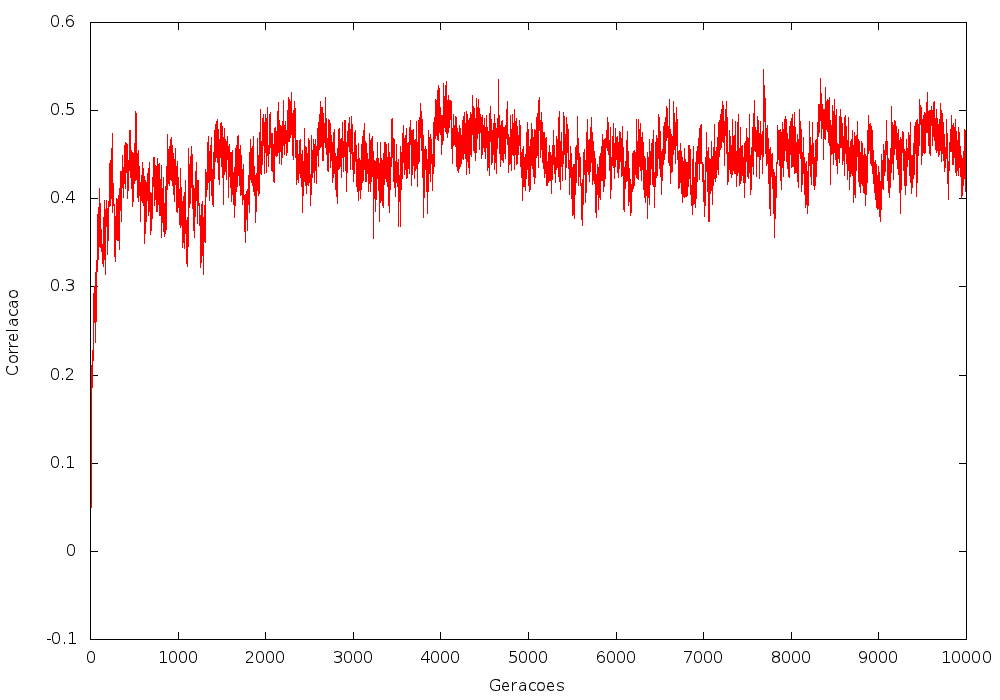
\includegraphics[width=150mm, height=80mm]{figuras/jones2tracos.png}
  \caption{Evolução da correlação entre dois traços ligados por efeitos
  mutacionais pleiotrópicos sobre seleção estabilizadora correlacionada.
  Nesta simulação $r_\omega=0.8$, $Ne=5000$, $p=2$, $m=50$}
  \label{jones2tracos}
\end{figure}
\end{center}

Como nosso objetivo é expandir a modelagem para mais traços, em seguida
adicionamos um traço ao sistema. Nesse caso, as considerações sobre a
dificuldade de manter a matriz $M$ positiva definida já se aplicam,
sendo necessário fazer uso da correção de auto-valores. Mesmo assim, o
resultado é bastante semelhante, ainda com a correlação entre os 3 traços
se alinhando com a matriz $\omega$ (figuras
\ref{jones3tracos} e \ref{MatJones3tracos}). 


\begin{center}
\begin{figure}[H]
  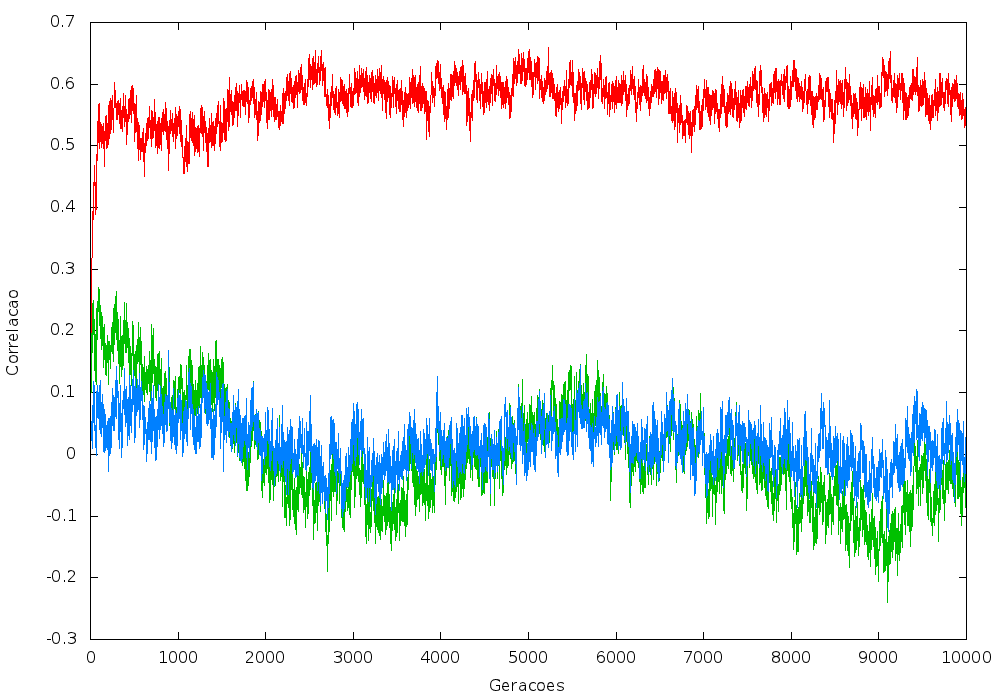
\includegraphics[width=150mm, height=80mm]{figuras/jones3tracos.png}
  \caption{Evolução da correlação entre três traços ligados por efeitos
  mutacionais pleiotrópicos sobre seleção estabilizadora correlacionada.
  A seleção propicia a integração entre dois traços (linha vermelha) e a desistegração
  desses dois com o terceiro (linhas azul e verde). Nesta simulação
  $r_\omega$ como na equação \ref{romega}, $Ne=5000$, $p=3$, $m=50$.}
  \label{jones3tracos}
\end{figure}
\end{center}

Na figura \ref{MatJones3tracos}
vemos representações gráficas da matriz de correlação fenotípica ao final da
simulação e da matriz $\omega$ de seleção estabilizadora correlacionada.
Caselas mais claras indicam correlação maior. Nesse caso a matriz de
correlação mutacional usada foi:

\begin{equation}
Corr(\omega) = \left( \begin{smallmatrix} 1 & 0.9 & 0.1\\  0.9 & 1 & 0.1 \\ 0.1 & 0.1 & 1 \end{smallmatrix}  \right)
\label{romega}
\end{equation}

E a matriz de covariância mutacional: 

\begin{equation}
\omega = \left( \begin{smallmatrix} 9 & 8.1 & 0.9\\  8.1 & 9 & 0.9 \\ 0.9 & 0.9 & 9 \end{smallmatrix}  \right)
\end{equation}

\begin{center}
\begin{figure}[H]
  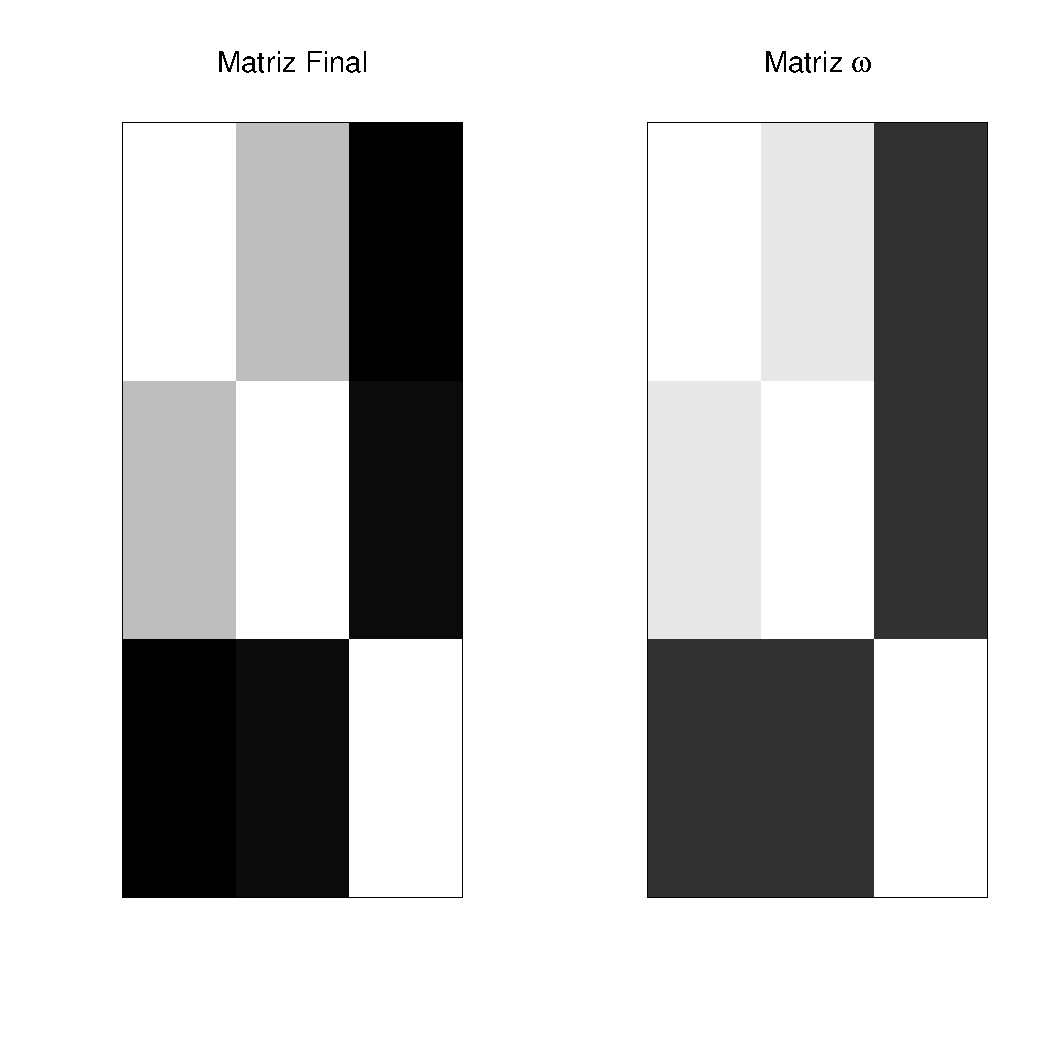
\includegraphics[width=150mm, height=80mm]{figuras/Mat3tracos}
   \caption{Comparação entre a matriz de correlação final para o 3
   traços após 10000
   gerações de seleção e a matriz $\omega$ da superfície de seleção.}
  \label{MatJones3tracos}
\end{figure}
\end{center}

Quando procuramos ampliar o número de traços, porém, o alinhamento da
matriz G com a matriz $\omega$ se mostrou problemático. Nesse caso a
matriz de correlação da superfície de seleção continha dois módulos, e
era dada por:

\begin{equation}
Corr(\omega) = \left( 
\begin{smallmatrix} 
1 & 0.8 & 0.8 & 0.8 & 0.8 & 0 & 0 & 0 & 0 & 0\\  
0.8 & 1 & 0.8 & 0.8 & 0.8 & 0 & 0 & 0 & 0 & 0\\  
0.8 & 0.8 & 1 & 0.8 & 0.8 & 0 & 0 & 0 & 0 & 0\\  
0.8 & 0.8 & 0.8 & 1 & 0.8 & 0 & 0 & 0 & 0 & 0\\  
0.8 & 0.8 & 0.8 & 0.8 & 1 & 0 & 0 & 0 & 0 & 0\\  
0 & 0 & 0 & 0 & 0 & 1 & 0.8 & 0.8 & 0.8 & 0.8\\ 
0 & 0 & 0 & 0 & 0 & 0.8 & 1 & 0.8 & 0.8 & 0.8\\
0 & 0 & 0 & 0 & 0 & 0.8 & 0.8 & 1 & 0.8 & 0.8\\
0 & 0 & 0 & 0 & 0 & 0.8 & 0.8 & 0.8 & 1 & 0.8\\
0 & 0 & 0 & 0 & 0 & 0.8 & 0.8 & 0.8 & 0.8 & 1
\end{smallmatrix}  \right)
\label{matw}
\end{equation}

Na figura \ref{jones10tracos} vemos a trajetória típica das correlações
fenotípicas com uma matriz $\omega$ com dois módulos (ver figura
\ref{MatJones10tracos}).  Aqui não existe mais a distinção entre
correlações dentro de módulos (altas) e entre módulos (baixas). Na figura
\ref{MatJones10tracos} fica claro que não existe semelhança entre as
matrizes G e $\omega$. Realizamos essas simulações com uma gama grande
de intensidades de seleção e chegando até 100000 gerações de seleção,
sem nenhum indício de alinhamento entre as matrizes $\omega$ e G.  

\begin{center}
\begin{figure}[H]
  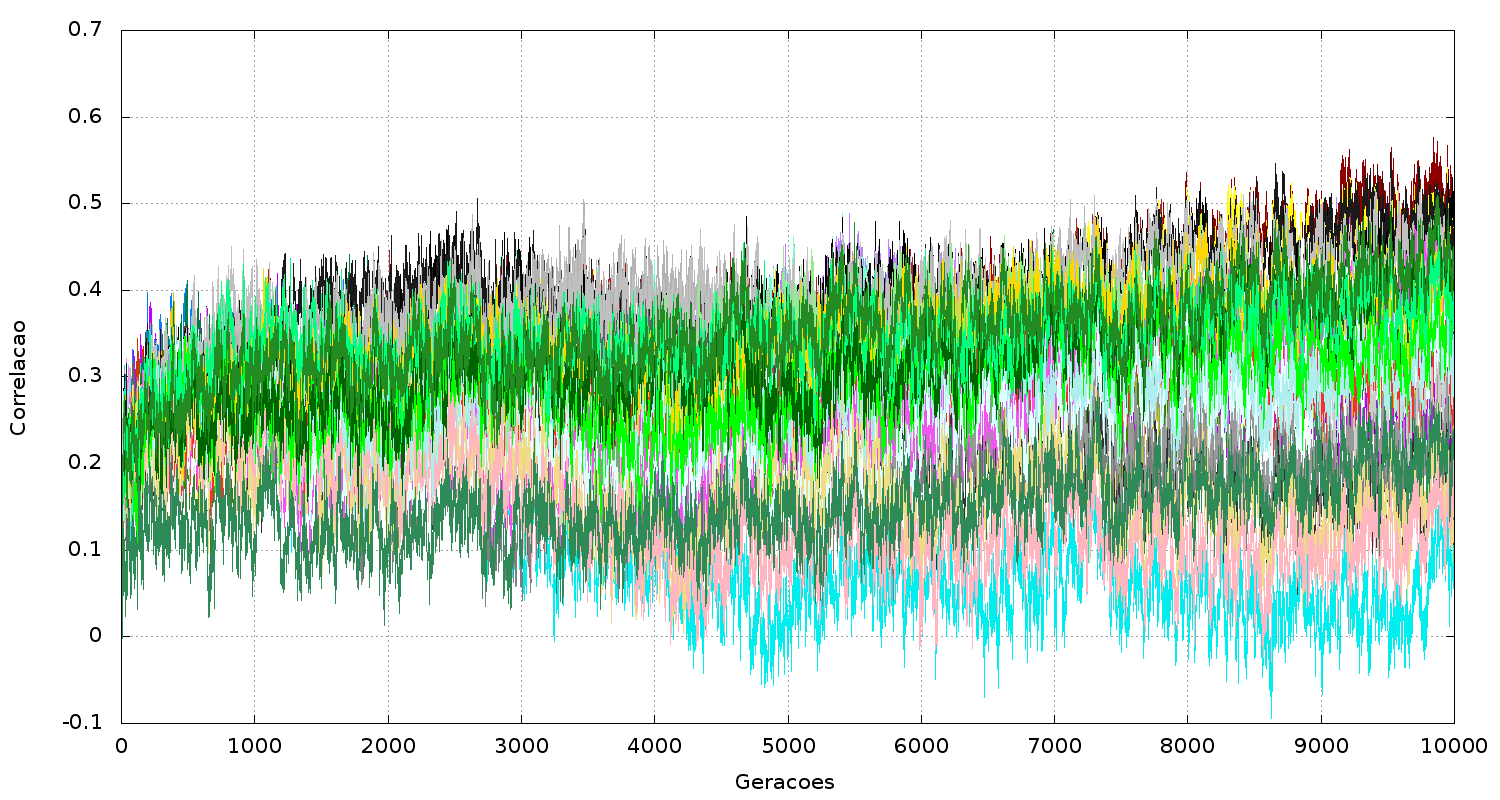
\includegraphics[width=150mm, height=80mm]{figuras/jones10tracos.png}
  \caption{Evolução da correlação entre dez traços ligados por efeitos
  mutacionais pleiotrópicos sobre seleção estabilizadora correlacionada.
  Apesar de a seleção promover a integração entre os 5 primeiros e os 5
  últimos traços e a desintegração entre esse módulos, isso não se
  transmite à matriz de correlação. Nesta simulação
    $r_\omega$ como na equação \ref{matw}, $Ne=5000$, $p=10$, $m=50$.}
  \label{jones10tracos}
\end{figure}
\end{center}

\begin{center}
\begin{figure}[H]
  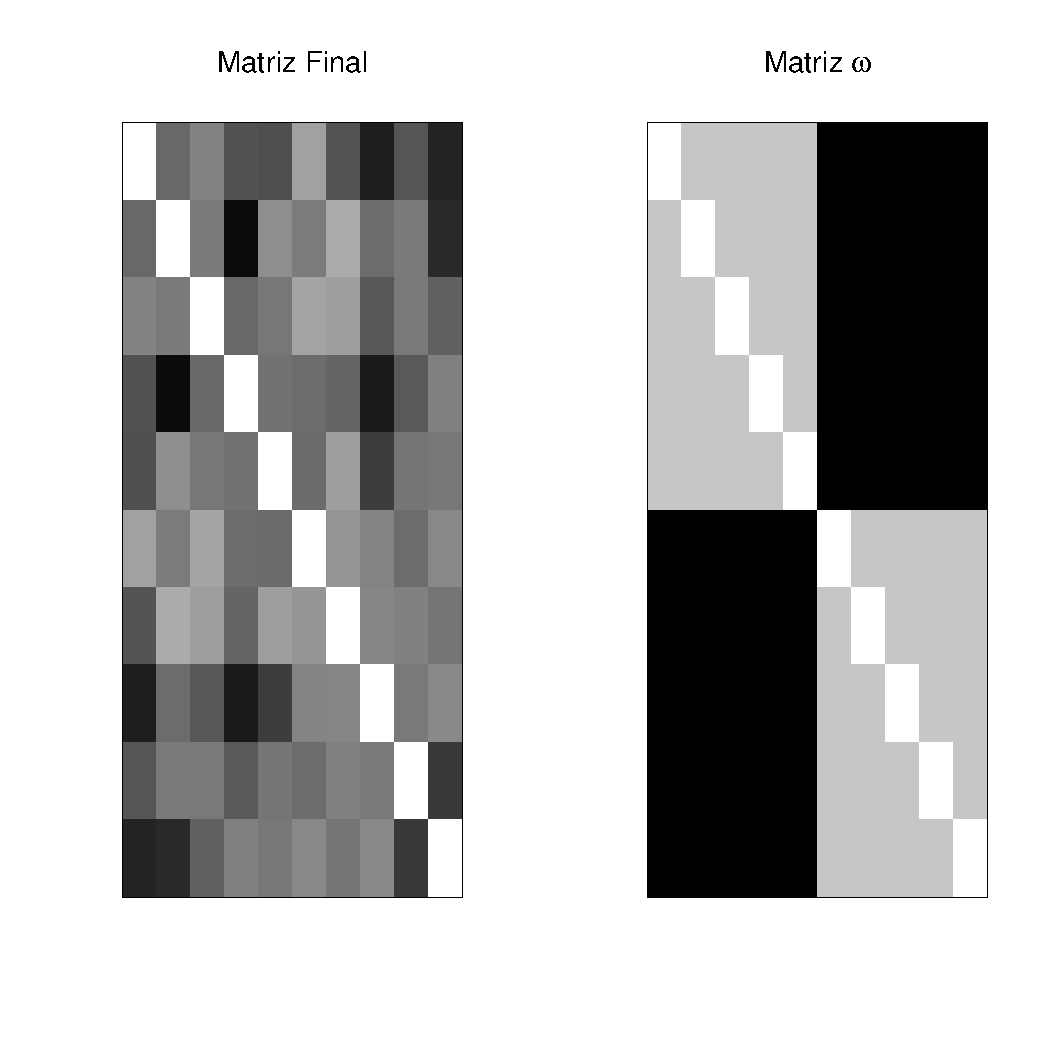
\includegraphics[width=150mm, height=80mm]{figuras/Mat10tracos}
  \caption{Comparação entre a matriz de correlação final para o 10 traços após 10000
   gerações de seleção representadas na figura \ref{jones10tracos} e a matriz $\omega$ da superfície de seleção.}
  \label{MatJones10tracos}
\end{figure}
\end{center}


\subsection{Seleção Direcional}

Em seguida, procuramos explorar como a inclusão de seleção direcional afetaria o
alinhamento das matrizes G e $\omega$. Utilizamos novamente uma matriz
$\omega$ modular e acresentamos seleção direcional correlacionada, de
mudança conjunta na média dos traços dentro de cada um dos módulos, e
mudanças antagônicas entre módulos. Ou seja, os 5 primeiros traços
tiveram seu ótimo fenotípico aumentado a uma taxa constante 
 e os 5 últimos traços tiveram seu ótimo reduzido de forma simétrica ($\Delta_S=0.2$).  As populações
respondem a essa seleção de forma satisfátoria, alterando suas médias de
acordo com a posição do ótimo. Após 10000 gerações de seleção
direcional,
nós observamos a matriz final e a evolução de todas as correlações
genéticas nesse período. Os resultados podem ser vistos nas figuras
\ref{jones10tracosDirecional} e \ref{MatJones10tracosDirecional}. Mesmo
nessas condições, não observamos a emergência de módulos variacionais na
matriz G, que indicaria semelhança com a matriz $\omega$ e o padrão de
seleção direcional correlacionada.

\begin{center}
\begin{figure}[H]
  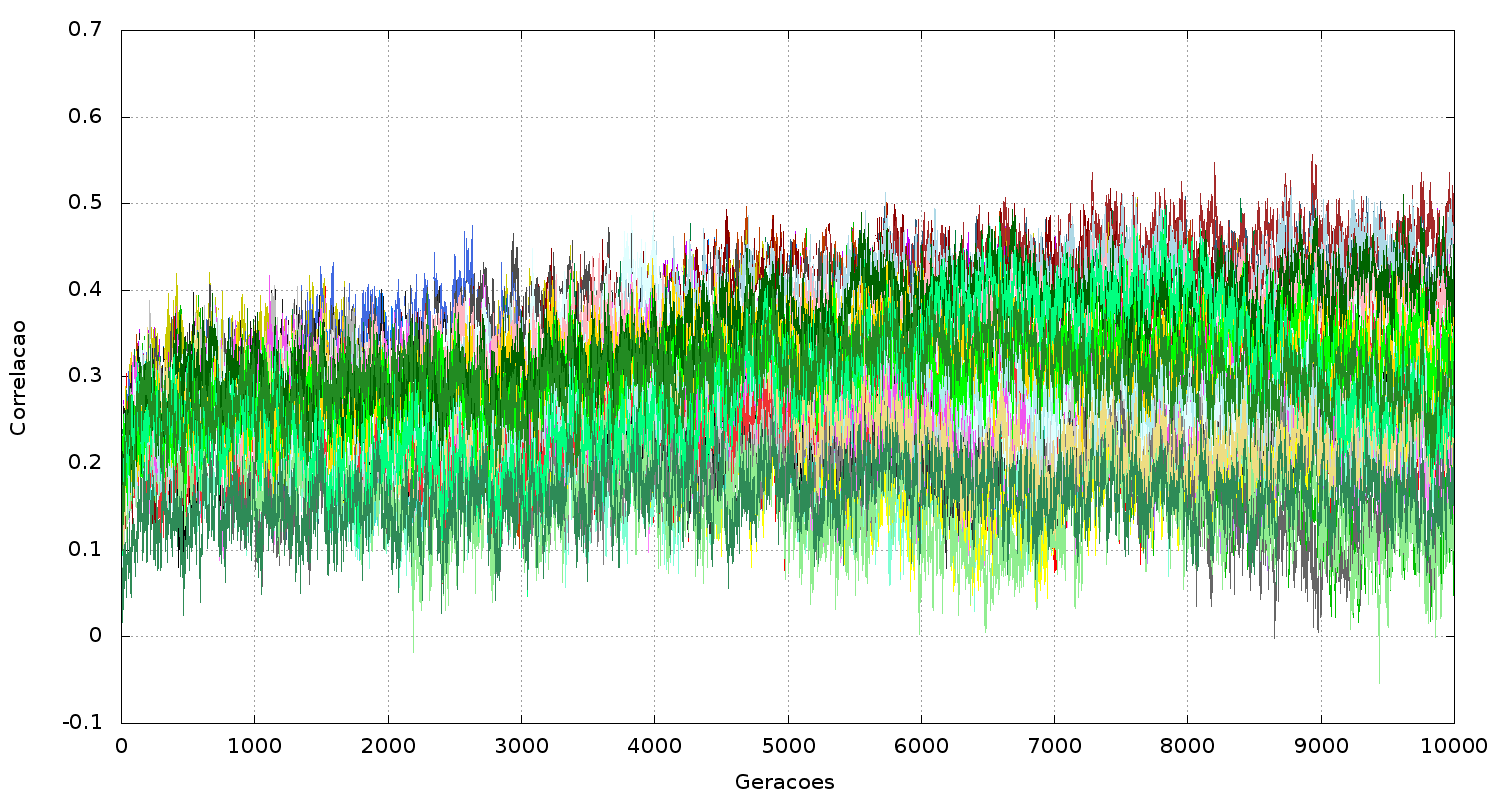
\includegraphics[width=150mm, height=80mm]{figuras/jones10tracosDirecional.png}
  \caption{Evolução da correlação entre dez traços ligados por efeitos
  mutacionais pleiotrópicos sobre seleção estabilizadora correlacionada
  e seleção direcional intensa para mudança correlacionada dentros dos
  módulos. Novamente, isso não se traduz na matriz de correlação genética.}
  \label{jones10tracosDirecional}
\end{figure}
\end{center}

\begin{center}
\begin{figure}[H]
  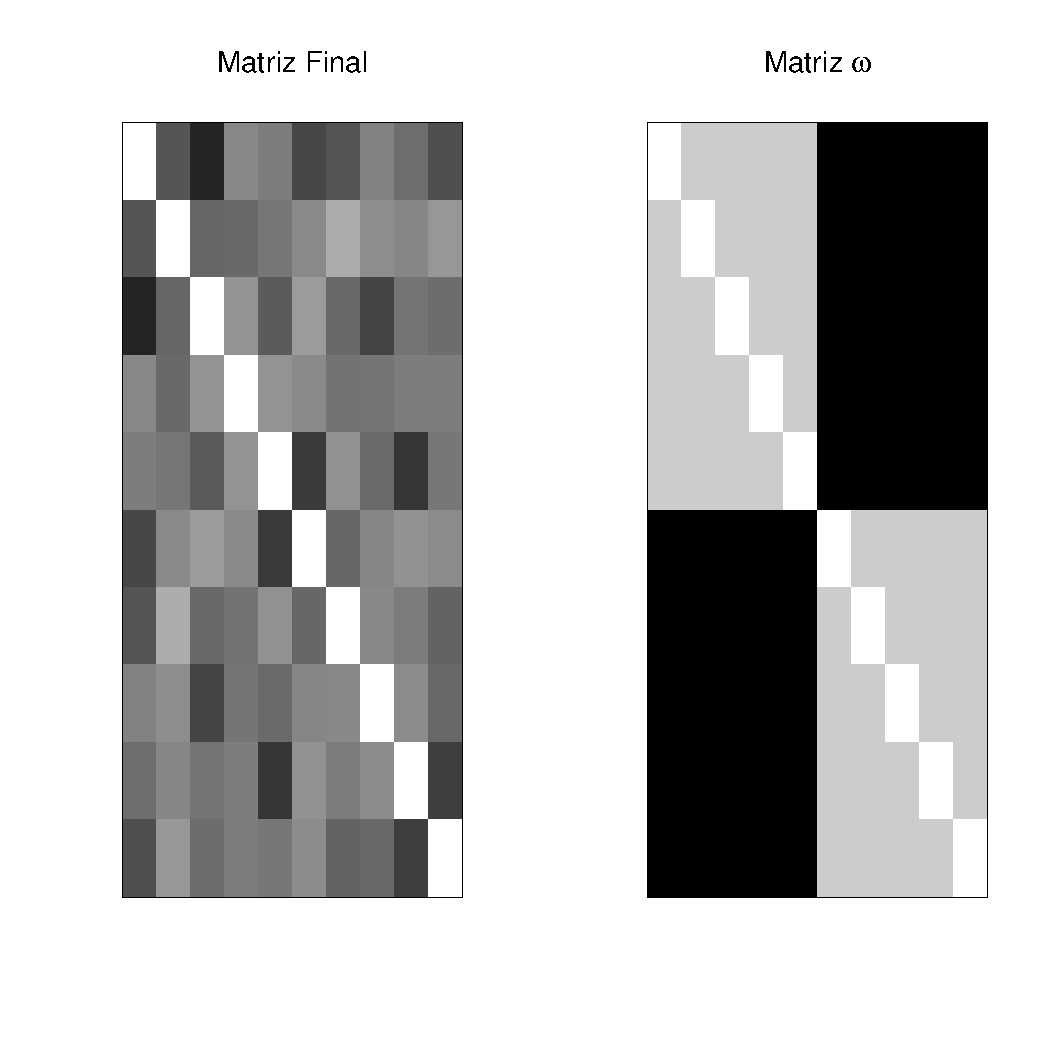
\includegraphics[width=150mm, height=80mm]{figuras/Mat10tracosDirecional}
   \caption{Comparação entre a matriz de correlação final para 10
   traços após 10000
   gerações de seleção direcional e estabilizadora representadas na figura \ref{jones10tracosDirecional} com a matriz $\omega$ da superfície de seleção.}
  \label{MatJones10tracosDirecional}
\end{figure}
\end{center}

Acreditamos que essa dificuldade em reproduzir os resultados encontrados
em sistemas com 2 e 3
traços no sistema com 10 traços se deve ao aumento considerável do
espaço possível de variação que a inclusão de cada novo traço
representa. O morfo-espaço cresce rapidamente com a inclusão de cada novo
traço, e as possibilidades para a matriz $M$ também. A seleção indireta
então se torna muito fraca para promover o alinhamento entre as
matrizes, e a mutação não explora de forma adequada o espaço da matriz
mutacional, levando a uma situação de não alinhamento mesmo com uma pressão
seletiva considerável.

\section{Resultados e Discussão $\cdot$ Matriz $B$}

\subsection{Seleção Estabilizadora}

No segundo tipo de modelagem, começamos já com 10 traços sofrendo
seleção estabilizadora correlacionada dada pela matriz apresentada na
equação \ref{matw}. Exploramos então a influência de várias razões entre
a taxa de mutação nos alelos aditivos ($\mu$) e a taxa de mutação nas
caselas da matriz $B$ ($\mu_B$).  Essa razão $\mu/\mu_B$ define como será a
dinâmica temporal de mudança entre dois níveis: o dos efeitos
aditivos e o da atribuição desses efeitos aos traços quantitativos.
Conforme vemos na figura \ref{MatBEstab}, apesar de mudanças na
magnitude das correlações com o aumento da razão $\mu/\mu_B$, não observamos o surgimento de módulos
variacionais apenas com seleção estabilizadora correlacionada.

\begin{center}
\begin{figure}[H]
  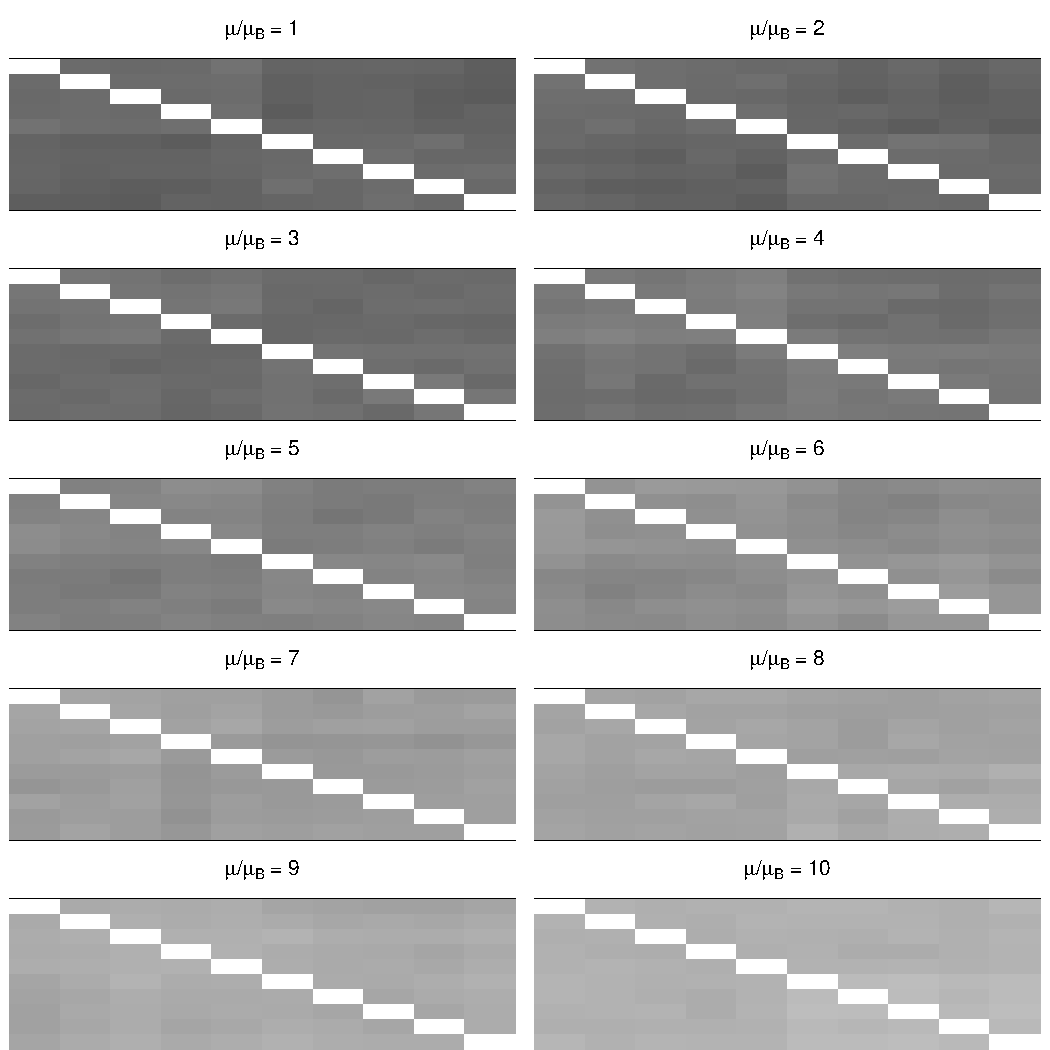
\includegraphics[width=150mm, height=180mm]{figuras/MatBEstabRMu}
   \caption{Matriz final média de 10 corridas para diferentes razões de
   $\mu$ e $\mu_B$, com seleção estabilizadora correlacionada com 2
   módulos.}
  \label{MatBEstab}
\end{figure}
\end{center}


\subsection{Seleção Direcional}

Com a inclusão de seleção direcional, como na figura
\ref{MatJones10tracosDirecional}, e $\mu/\mu_B = 0.1$, ainda não
observamos a formação de módulos na matriz G (figura \ref{RMu01}). 

\begin{center}
\begin{figure}[H]
  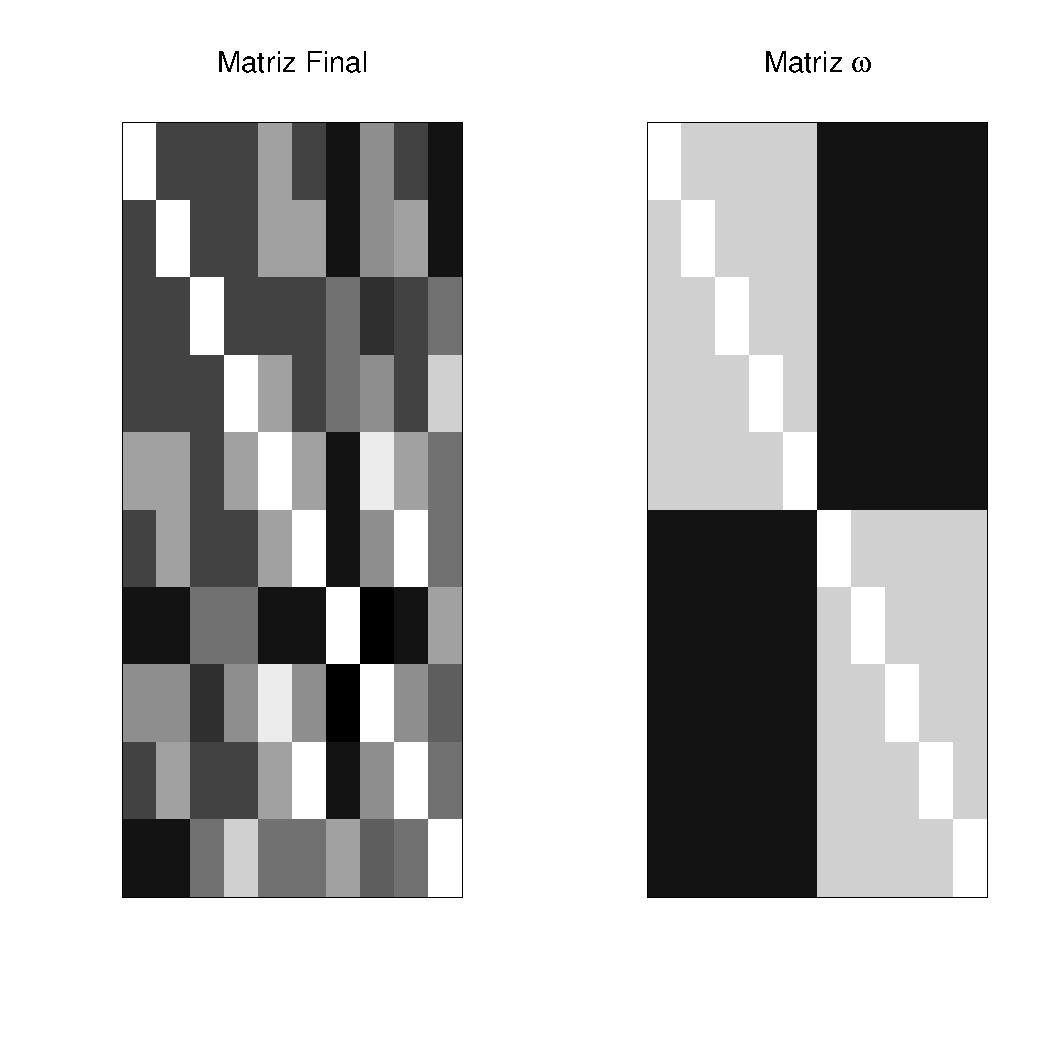
\includegraphics[width=150mm, height=80mm]{figuras/RMu01Omega}
   \caption{Comparação entre a matriz de correlação final média de 10
   corridas para o 10 traços após 10000
   gerações de seleção direcional e estbilizadora com a matriz $\omega$ da superfície de seleção e $\frac{\mu}{\mu_B}=0.1$, $Ne=2500$, $\Delta_S=0.2$, $m/p=2$}
  \label{RMu01}
\end{figure}
\end{center}

Porém, como vemos na figura \ref{MatBDirecional-RMu}, o aumento  na
razão $\mu/\mu_B$ aliada à seleção direcional é capaz de alterar essa
situação. Esse aumento parece promover um sistema capaz de responder de
forma eficiente às pressões seletivas impostas e gerar uma matriz G com
a estrutura modular privilegiada pela seleção estabilizadora e
direcional. Lembramos que na ausência de seleção direcional esse efeito
não é observado, mesmo com as mesmas razões $\mu/\mu_B$.  Além disso,
parece haver um pico na modularidade das matrizes com $\mu/\mu_B = 5$,
sugerindo uma possível otimização entre a escala temporal de mudança em cada
nível de complexidade, porém isso deve ser confirmado com mais corridas
e com diferentes combinações de parâmetros de tamanho populacional,
força de seleção e número de alelos aditivos.

Na figura \ref{MatBDirecionalNe2500RMu5} vemos um exemplo de corrida com
$N_e = 2500$ e $\mu/\mu_B=5$, mostrando claramente a separação de grupos
de correlação dentro de e entre módulos. Posteriormente, vamos explorar a
influência do tamanho populacional na estabilidade das matrizes geradas
pelas nossas simulações (figura \ref{posselecao}).

\begin{center}
\begin{figure}[H]
  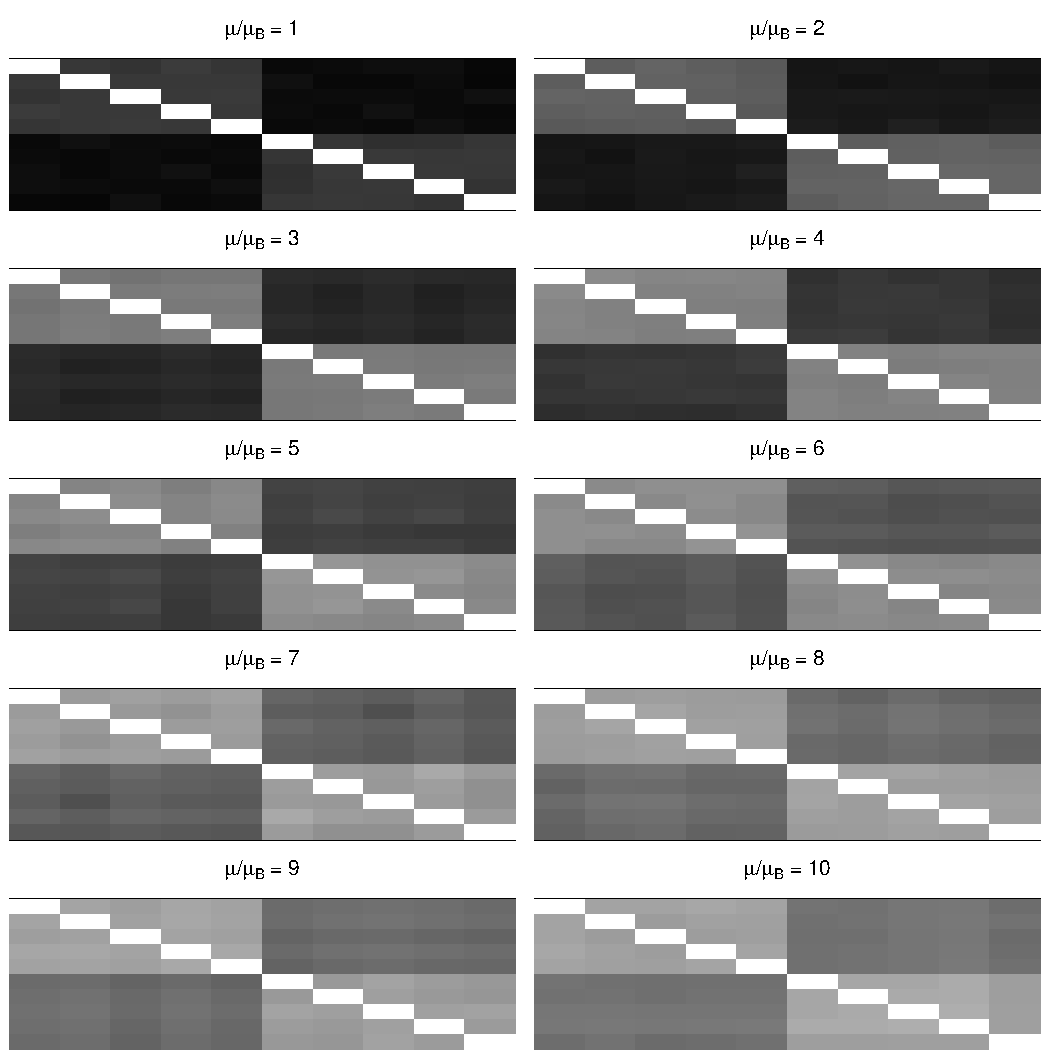
\includegraphics[width=150mm, height=180mm]{figuras/MatBDirecRMu}
   \caption{Matriz final média de 10 corridas para diferentes razões de
   $\frac{\mu}{\mu_B}$, com seleção estabilizadora correlacionada com 2
   módulos e seleção direcional correlacionada favorecendo os mesmos
   módulos. ($N_e=2500$, $\Delta_S=0.2$, $m/n=2$)}
  \label{MatBDirecional-RMu}
\end{figure}
\end{center}

\begin{center}
\begin{figure}[H]
  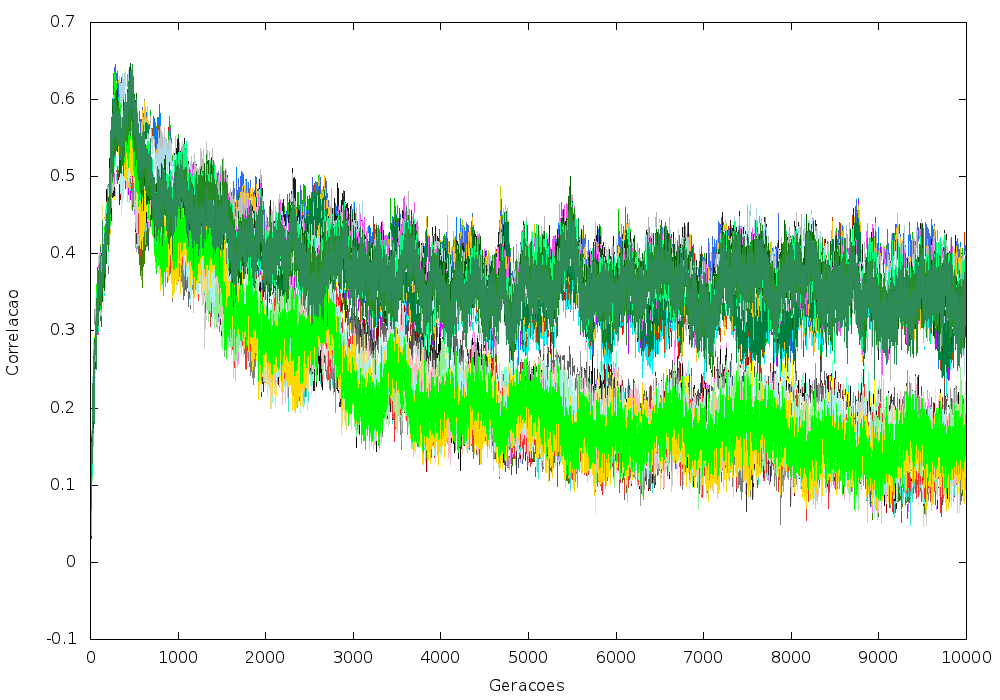
\includegraphics[width=150mm, height=80mm]{figuras/direcionalNe2500RMu5.png}
  \caption{Evolução da correlação entre dez traços ligados por efeitos
  pleiotrópicos controlados por uma função ontogenética linear binária
  variável, sofrendo seleção estabilizadora correlacionada
  e seleção direcional intensa para mudança correlacionada dentros dos
  módulos durante as 10000 gerações. 
  ($N_e = 2500$, $\mu/\mu_B=5$, $\Delta_S=0.2$, $m/p=2$)}
  \label{MatBDirecionalNe2500RMu5}
\end{figure}
\end{center}

Estamos interessados também na força de seleção direcional
necessária para gerar a estrutura modular nas matrizes de covariação.
Nas figuras \ref{MatBIntSel110} e \ref{MatBIntSel1120} vemos matrizes
médias finais para 10 corridas com $N_e = 1000$, $\mu/\mu_B=5$ e intensidade de
seleção variável. 

Para isso, modificamos o quanto o pico adaptativo era
alterado para cada traço a cada geração, de $0.01$ até $0.2$ por
geração durante 10000 gerações. 

A medida que aumentamos a intensidade de seleção os modulos se tornam
mais evidentes, mas acima de uma certa intensidade (delta $\simeq 0.06$)
esse efeito se torna mais discreto.  Esse platô na resposta a seleção
direcional pode ser explicado por como funciona a nossa seleção. Quando
a variância entre as aptidões na população for suficientemente alta,
apenas os indivíduos com maior aptidão vão se reproduzir, e, dentro de
limites\footnote{ Quando o pico se encotra suficientemente longe da média
da população, a variância nos valores de aptidão cai novamente, pois
todos os indivíduos tem aptidão próxima de zero, e a chance de um
indivíduo se reproduzir deixa de depender do fenótipo. Isso é uma
limitação do esquema de seleção estritamente gaussiano.}, as mudanças em
$\Delta_S$ não alteram quais são esses indivíduos.

\begin{center}
\begin{figure}[H]
  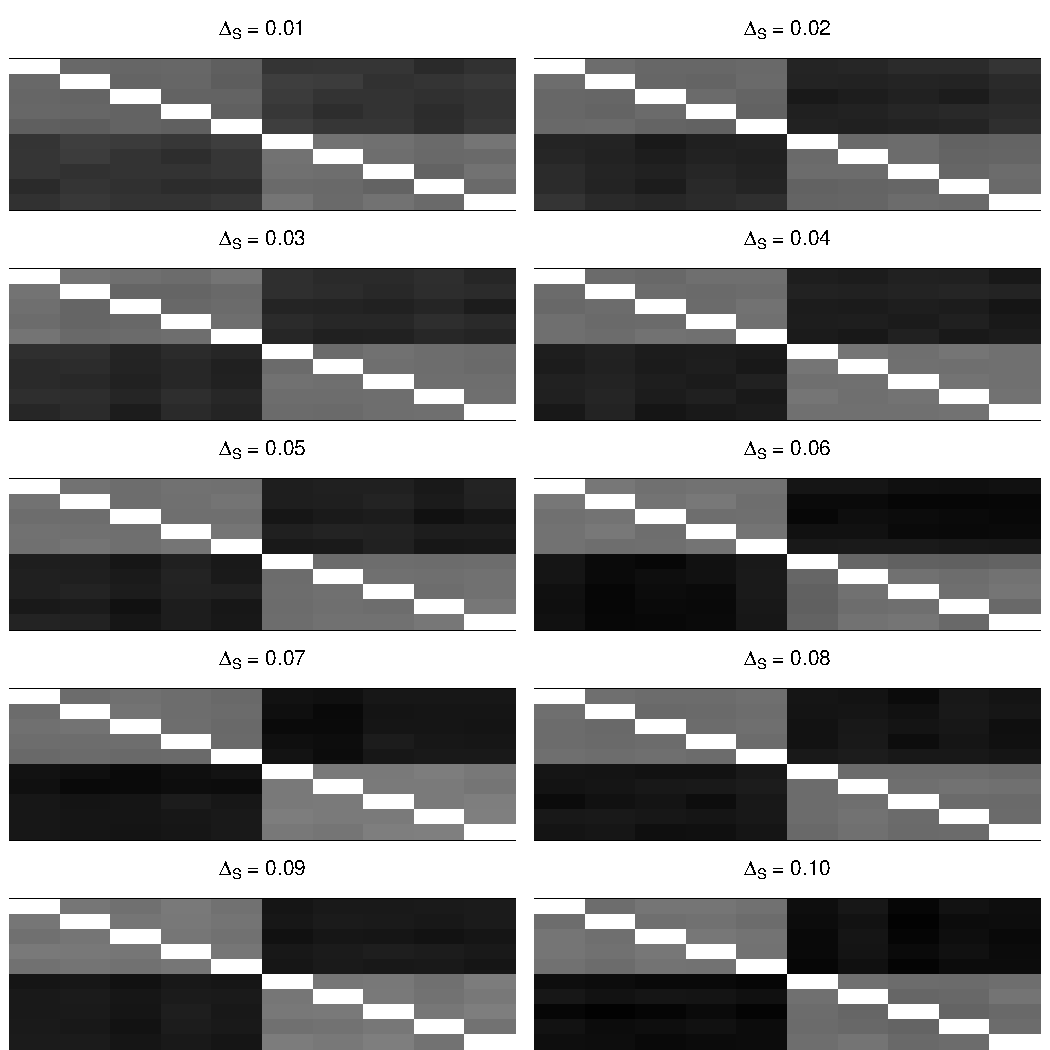
\includegraphics[width=150mm, height=180mm]{figuras/MatBDirecionalIntSel110}
   \caption{Matriz final média de 10 corridas com
   $\frac{\mu}{\mu_B} = 5$, $Ne = 1000$, $m/p=2$, sofrendo seleção estabilizadora correlacionada com 2
   módulos e seleção direcional com diferentes valores de $\Delta_S$.}
  \label{MatBIntSel110}
\end{figure}
\end{center}

\begin{center}
\begin{figure}[H]
  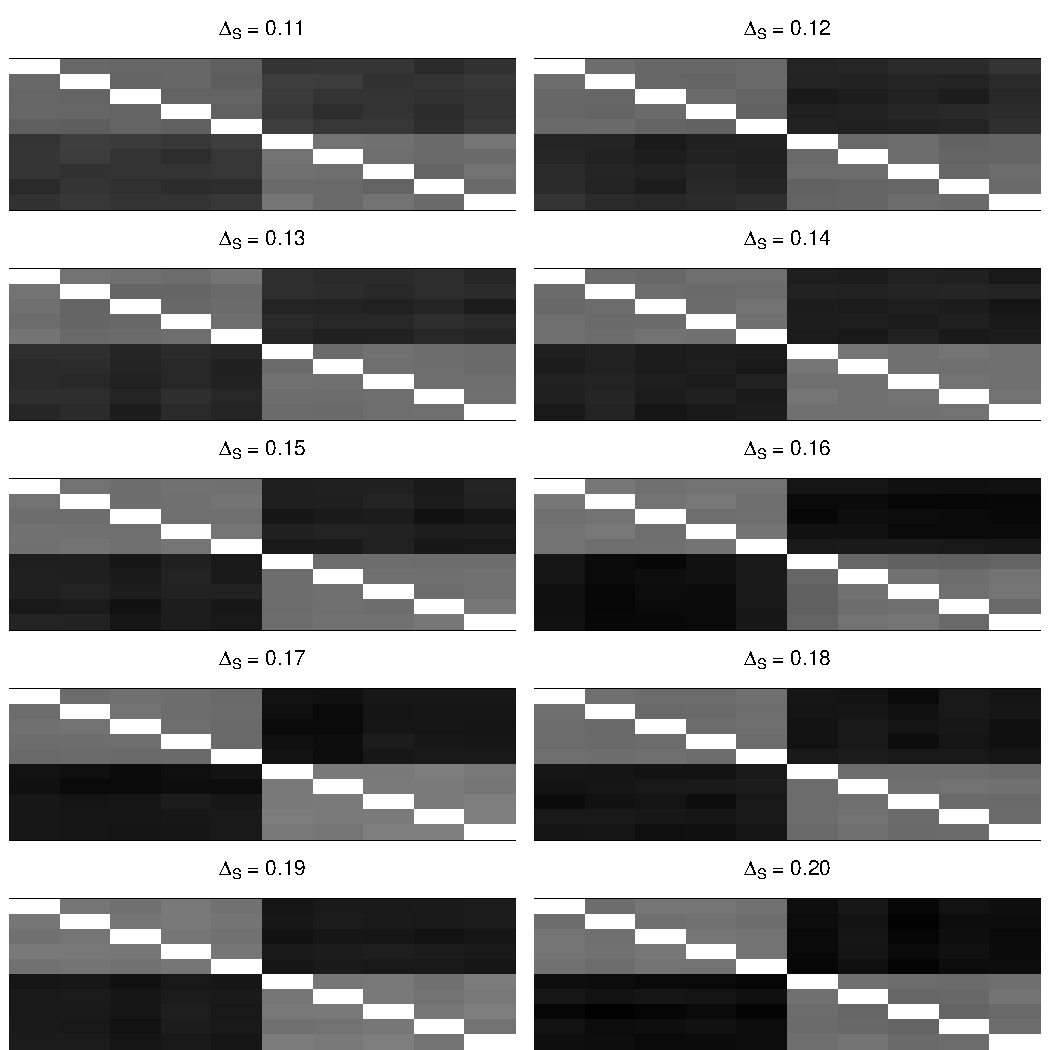
\includegraphics[width=150mm, height=180mm]{figuras/MatBDirecionalIntSel1120}
   \caption{Matriz final média de 10 corridas com
   $\frac{\mu}{\mu_B} = 5$, $Ne = 1000$, $m/p=2$, sofrendo seleção estabilizadora correlacionada com 2
   módulos e seleção direcional com diferentes valores de $\Delta_S$.}
  \label{MatBIntSel1120}
\end{figure}
\end{center}

Outra questão relevante é o quão estáveis são os padrões de covariação
modulares gerados pela seleção direcional e estabilizadora.  Para
responder a essa pergunta nós sujeitamos populações de tamanhos
diferentes a uma mesma pressão seletiva intensa durante 5000 gerações
(periodo suficiente para o surgimento de módulos), seguidas de 5000
gerações de seleção estabilizadora correlacionada. Apesar da diferença
entre as correlações dentro e entre modulos diminuir, ainda observamos
uma distinção estável entre elas (figura \ref{posselecao}). O efeito do
tamanho populacional é especialmente marcante nessas condições, com
populações grandes se mostrando mais eficientes na manutenção prolongada
dos padrões estabelecidos pela seleção direcional (figura
\ref{posselecao}).

\begin{center}
\begin{figure}[H]
  \subfloat [$Ne = 250$]{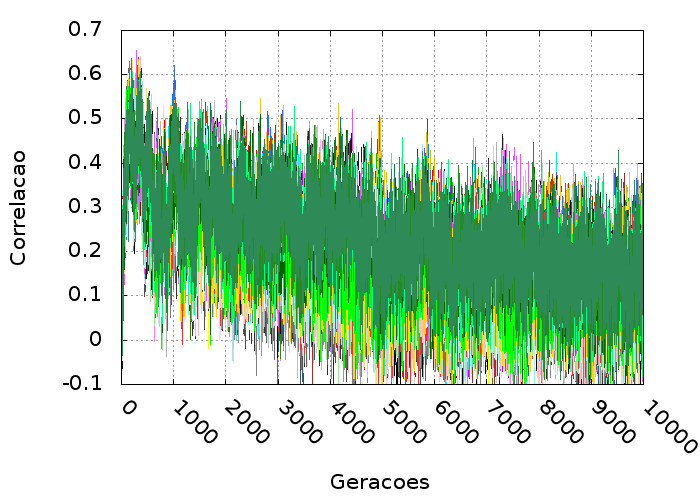
\includegraphics[width=50mm, height=80mm]{figuras/posselecao250.png}}
  \subfloat [$Ne = 500$]{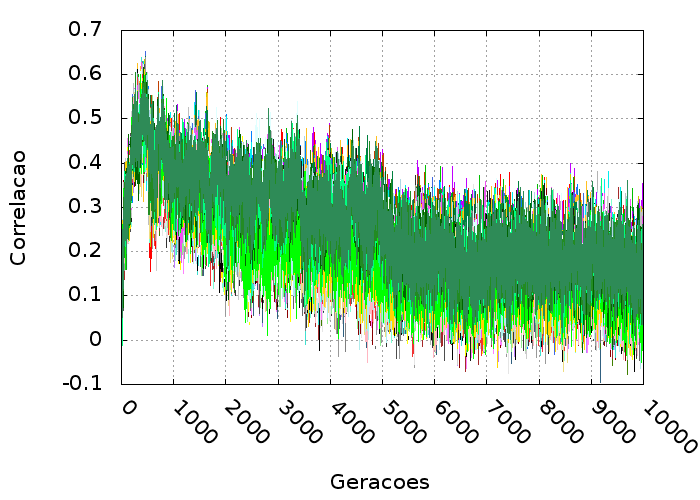
\includegraphics[width=50mm, height=80mm]{figuras/posselecao500.png}}
  \subfloat [$Ne = 1000$]{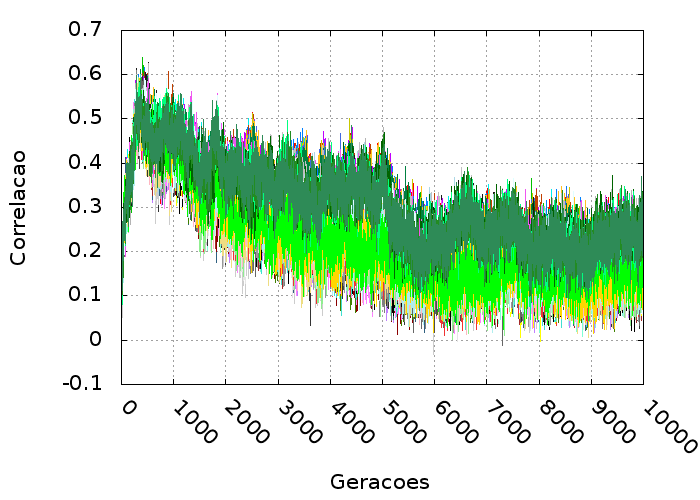
\includegraphics[width=50mm, height=80mm]{figuras/posselecao1000.png}}
\end{figure}
\begin{figure}[H]
  \subfloat [$Ne = 2500$]{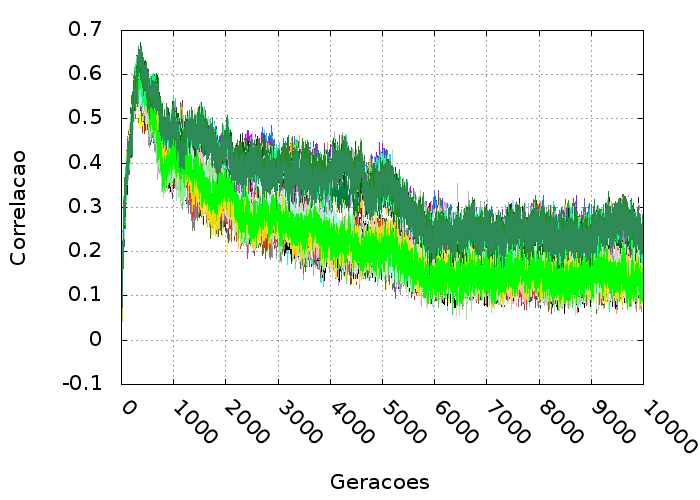
\includegraphics[width=50mm, height=80mm]{figuras/posselecao2500.png}}
  \subfloat [$Ne = 5000$]{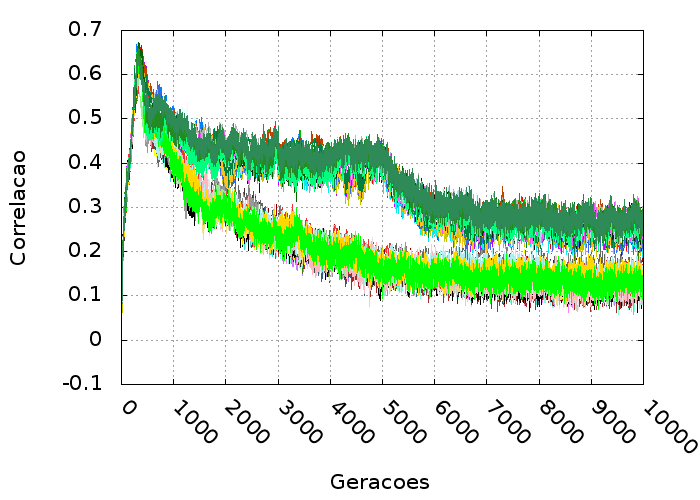
\includegraphics[width=50mm, height=80mm]{figuras/posselecao5000.png}}
  \subfloat [$Ne = 10000$]{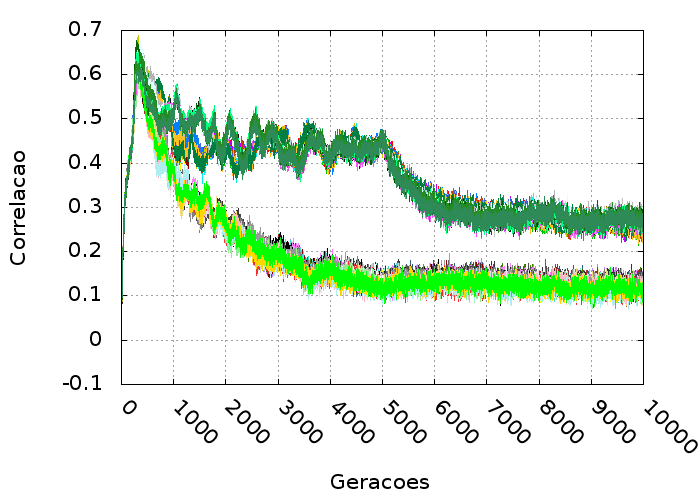
\includegraphics[width=50mm, height=80mm]{figuras/posselecao10000.png}}
  \caption{Evolução da correlação entre dez traços ligados por efeitos
  pleiotrópicos controlados por uma matriz $B$ variável, sofrendo seleção estabilizadora correlacionada e seleção
  direcional para mudança correlacionada dentros dos módulos
  durante as 5000 primeiras gerações, seguidos de 5000 gerações de
  seleção estabilizadora correlacionada ($\Delta_S = 0.2$, $\mu/\mu_B=5$, $m/p=2$). }
  \label{posselecao}
\end{figure}
\end{center}


\begin{center}
\begin{figure}[H]
  \subfloat [$Ne = 250$]{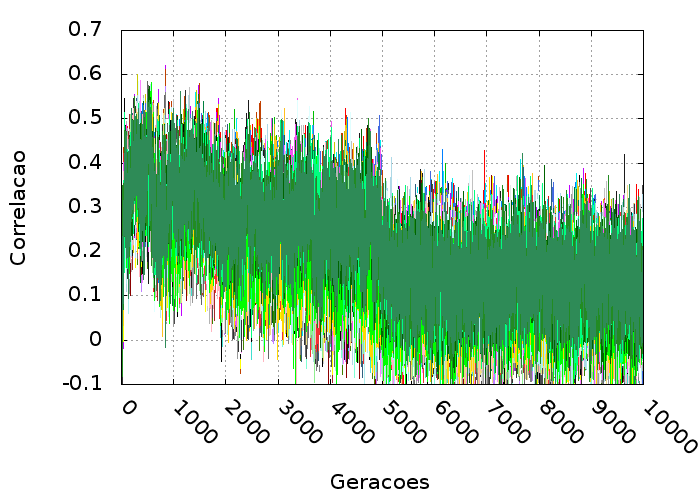
\includegraphics[width=50mm, height=80mm]{figuras/posselecaoSemEstab250.png}}
  \subfloat [$Ne = 500$]{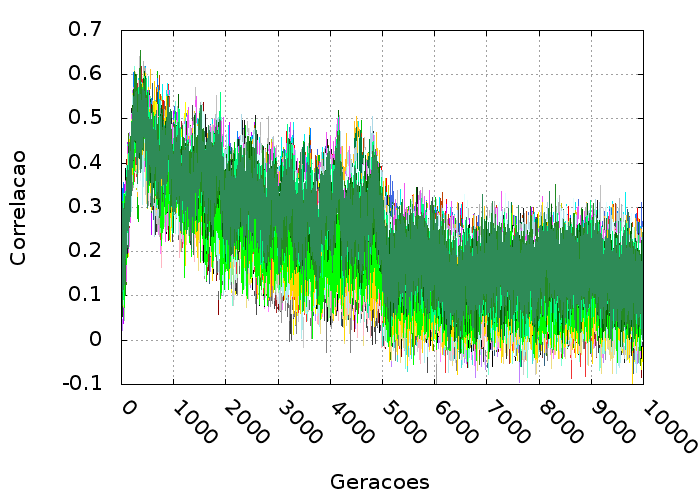
\includegraphics[width=50mm, height=80mm]{figuras/posselecaoSemEstab500.png}}
  \subfloat [$Ne = 1000$]{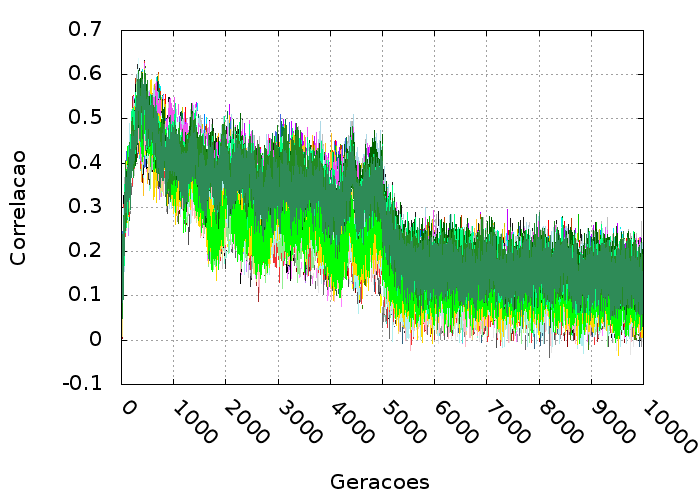
\includegraphics[width=50mm, height=80mm]{figuras/posselecaoSemEstab1000.png}}
\end{figure}
\begin{figure}[H]
  \subfloat [$Ne = 2500$]{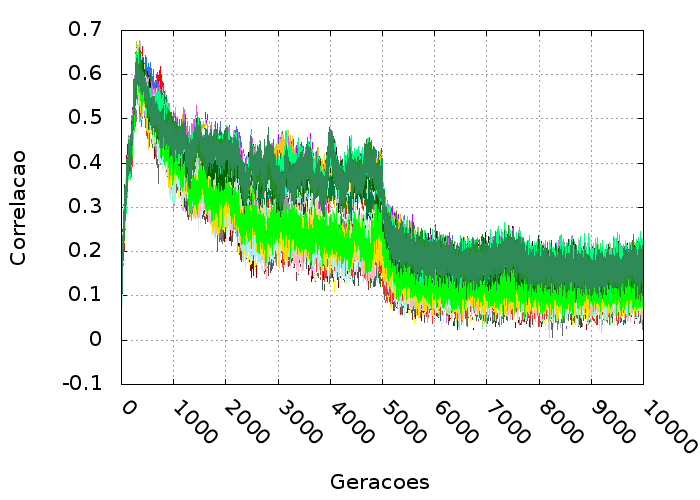
\includegraphics[width=50mm, height=80mm]{figuras/posselecaoSemEstab2500.png}}
  \subfloat [$Ne = 5000$]{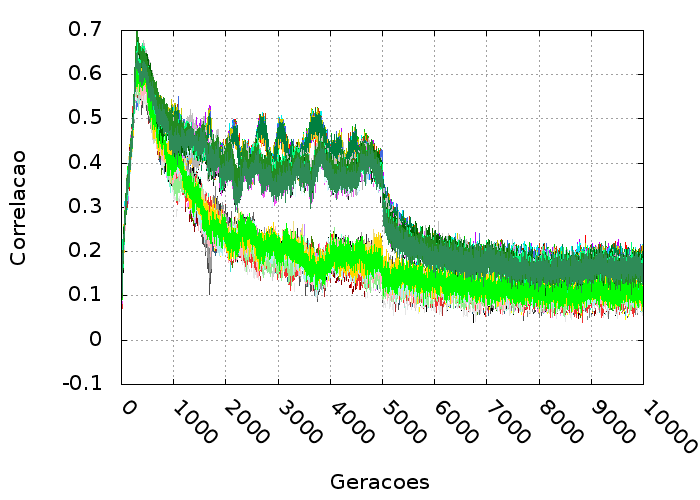
\includegraphics[width=50mm, height=80mm]{figuras/posselecaoSemEstab5000.png}}
  \subfloat [$Ne = 10000$]{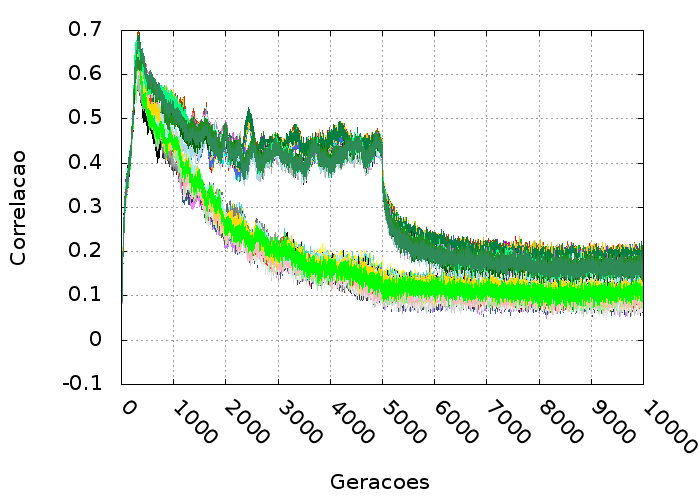
\includegraphics[width=50mm, height=80mm]{figuras/posselecaoSemEstab10000.png}}
  \caption{Evolução da correlação entre dez traços ligados por efeitos
  pleiotrópicos controlados por uma matriz $B$ variável, sofrendo seleção estabilizadora correlacionada e seleção
  direcional para mudança correlacionada dentros dos módulos
  durante as 5000 primeiras gerações, seguidos de 5000 gerações de
  seleção estabilizadora não correlacionada ($\Delta_S = 0.2$, $\mu/\mu_B=5$, $m/p=2$). }
  \label{posselecaoSemEstab}
\end{figure}
\end{center}

Ainda na questão da estabilidade dos padrões de covariação, o papel da
seleção estabilizadora correlacionada pode ser avaliado sujeitando as
populações à seleção direcional e estabilizadora correlacionada por 5000
gerações, seguidas de 5000 gerações de seleção estabilizadora não
correlacionada, apenas mantendo a média de cada traço individualmente.
Na figura \ref{posselecaoSemEstab} podemos ver a importância da seleção
estabilizadora correlacionada na manutenção dos padrões modulares
gerados pela seleção direcional. Comparando cada tamanho populacional
mostrado nas figuras \ref{posselecao} e \ref{posselecaoSemEstab} podemos
ver uma degradação muito mais acentuada dos padrões modulares na
ausência da seleção estabilizadora correlacionada. 

A importância da seleção estabilizadora para explicar padrões de estase
no registro fóssil foi amplamente discutida em \cite{Charlesworth1982a}.
No contexto de padrões de covariação, seleção estabilizadora
correlacionada também foi apontada como uma provável explicação para 
a estabilidade de padrões de covariação observados na natureza
\citep{Cheverud1984, Marroig2001, Porto2008}. Nossos resultados dão
credibilidade a essa hipótese. A origem dessa seleção estabilizadora
pode ser atribuida a fatores internos dos organismos, como restrições
ontogenéticas responsáveis pela coesão entre as partes do indivíduo.
Como essas restrições estão sempre presentes, a seleção correlacionada
está sempre presente e os padrões tendem a se manter estáveis.

Um parâmetro ainda não mencionado é o número de alelos $m$ envolvidos na
determinação do valor fenotípico de cada um dos $p$ traços. No nosso
esquema de simulação, aumentar o valor da razão $m/p$ é análogo a
aumentar a força de recombinação, pois o valor de $m$ define o número de unidades
recombinantes segregando na população. Podemos pensar em $m$ como o
número de cromossomos no genôma do indivíduo, em vez de pensar nele como
número de alelos individualmente. Até agora a razão $m/p$ foi mantida em
2, um valor suficiente para promover respostas complexas de todos os
traços mas ainda computacionalmente viável. A figura \ref{MB} mostra como o
aumento na razão $m/p$ afeta a evolução das correlações fenotípicas nas
populações sujeitas a seleção direcional intensa e seleção
estabilizadora correlacionada. 

\begin{center}
\begin{figure}[H]
  \subfloat [$m/p = 2$]{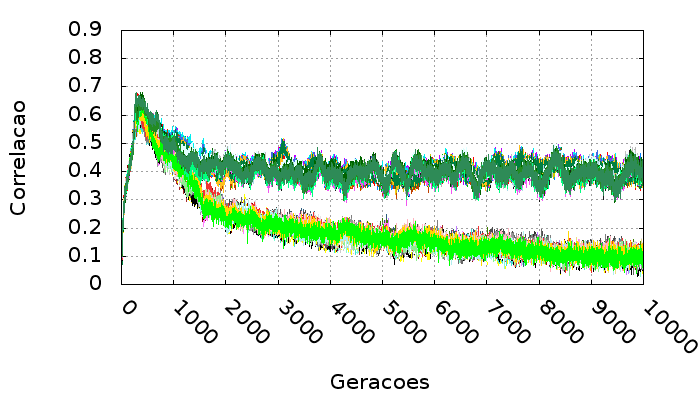
\includegraphics[width=50mm, height=55mm]{figuras/MB20.png}}
  \subfloat [$m/p = 3$]{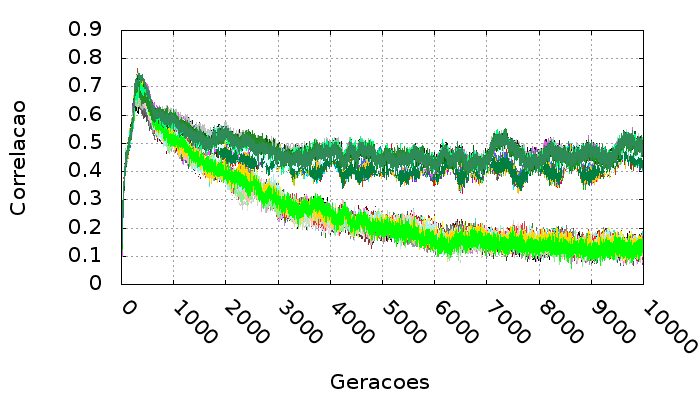
\includegraphics[width=50mm, height=55mm]{figuras/MB30.png}}
  \subfloat [$m/p = 4$]{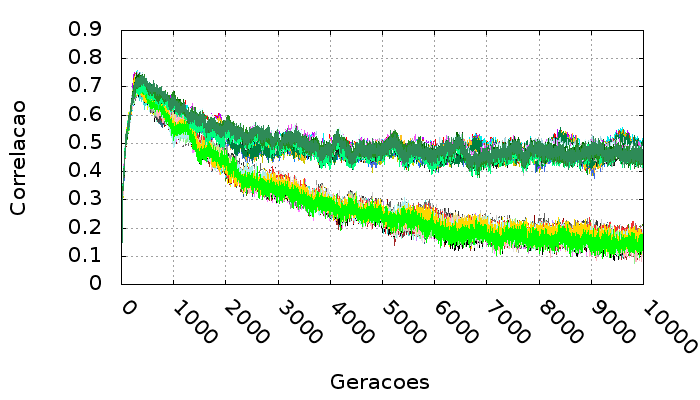
\includegraphics[width=50mm, height=55mm]{figuras/MB40.png}}
\end{figure}
\begin{figure}[H]
  \subfloat [$m/p = 5$]{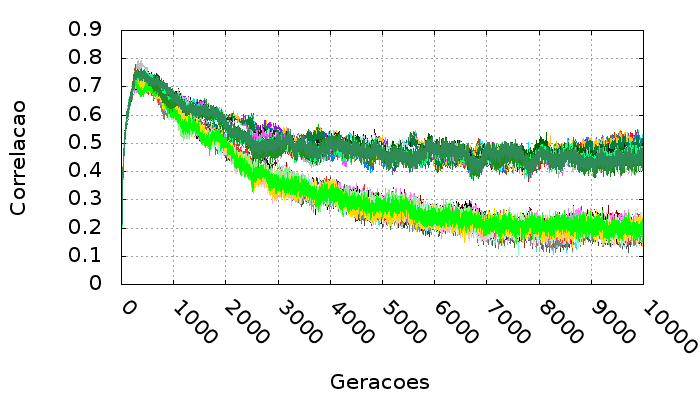
\includegraphics[width=50mm, height=55mm]{figuras/MB50.png}}
  \subfloat [$m/p = 6$]{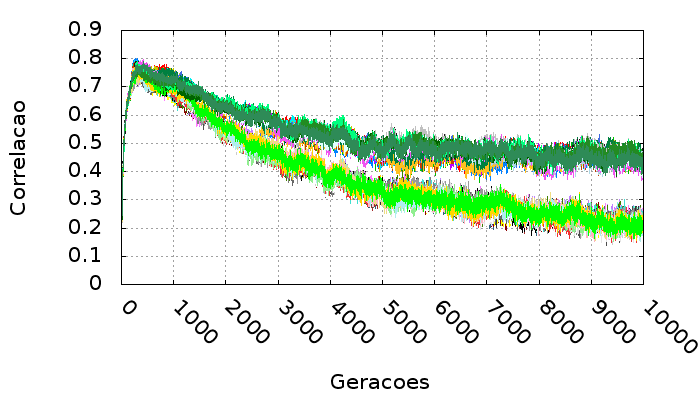
\includegraphics[width=50mm, height=55mm]{figuras/MB60.png}}
  \subfloat [$m/p = 7$]{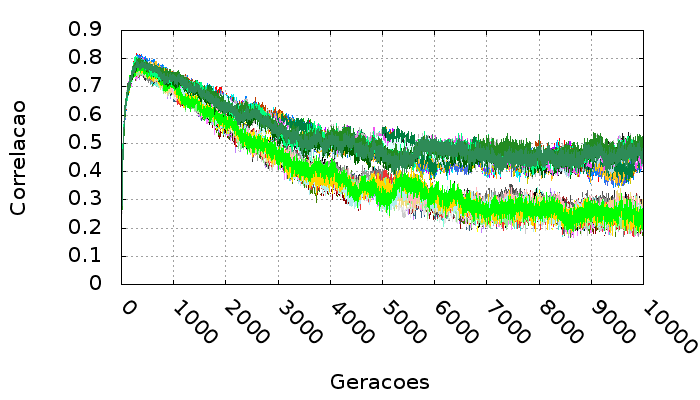
\includegraphics[width=50mm, height=55mm]{figuras/MB70.png}}
\end{figure}
\begin{figure}[H]
  \subfloat [$m/p = 8$]{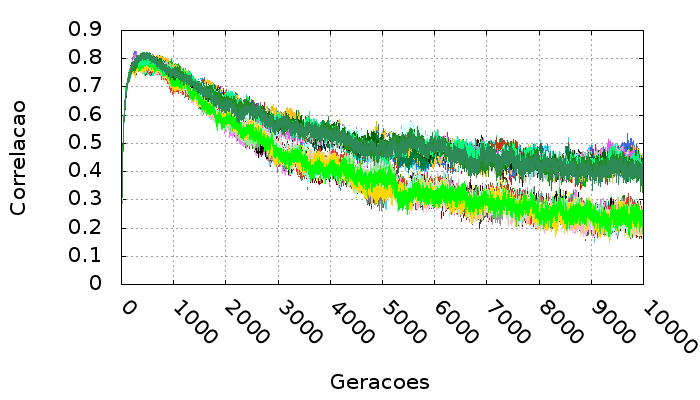
\includegraphics[width=50mm, height=55mm]{figuras/MB80.png}}
  \subfloat [$m/p = 9$]{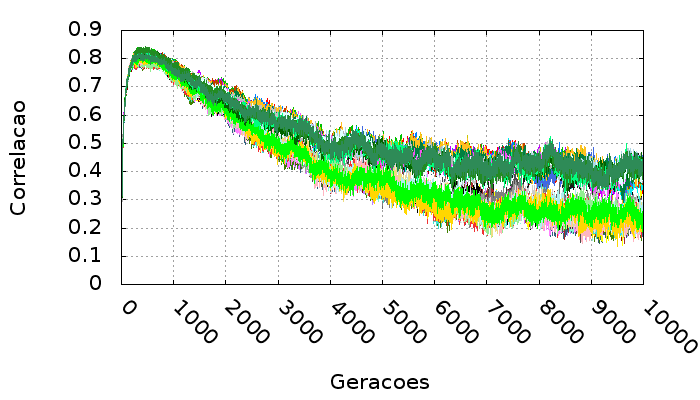
\includegraphics[width=50mm, height=55mm]{figuras/MB90.png}}
  \subfloat [$m/p = 10$]{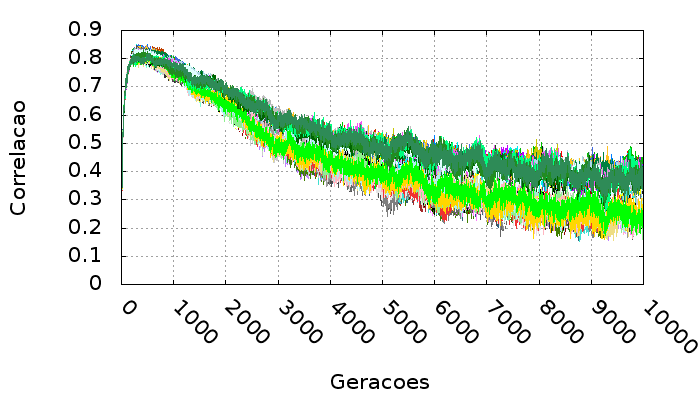
\includegraphics[width=50mm, height=55mm]{figuras/MB100.png}}
  \caption{Evolução da correlação entre dez traços ligados por efeitos
  pleiotrópicos controlados por uma função ontogenética linear binária
  variável sofrendo seleção estabilizadora correlacionada e seleção
  direcional intensa para mudança correlacionada dentros dos módulos,
  para diferentes valores do número de alelos. ($Ne=5000$, $\mu/\mu_B=5$, $\Delta_S=0.2$)}
  \label{MB}
\end{figure}
\end{center}

Vemos na figura \ref{MB} que o aumento do número de alelos torna o
sistema mais lento em adquirir um caráter modular. Isso pode ser
associado com o aumento na recombinação, que age na direção oposta a das
forças seletivas direcionais e estabilizadora correlacionada. Isso nos
levou a crer que tempos mais longos de seleção poderiam gerar o mesmo
resultado que o obtido com valores baixos de $m/p$. Na figura \ref{MBLR}
vemos duas corridas longas, de 20000 gerações, com $m/p = 9$ e $10$,
mostrando o tempo de estabilização mais longo e a modularidade mais
discreta, com menor diferença nas correlações dentro de e entre módulos.
Isso pode ser associado à força de recombinação aumentada.

\begin{center}
\begin{figure}[H]
  \subfloat [$m/p = 9$]{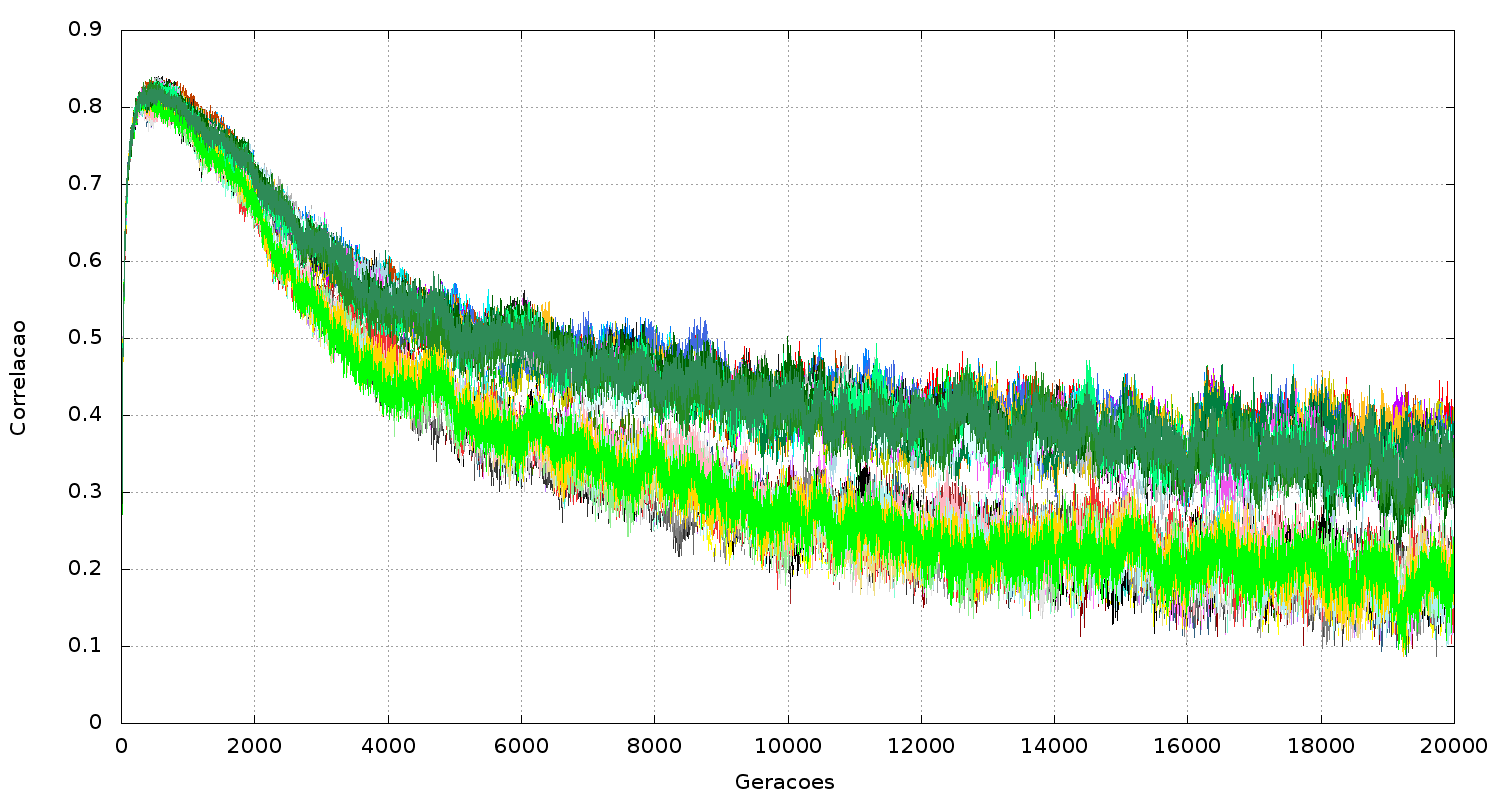
\includegraphics[width=150mm, height=55mm]{figuras/MBLR90.png}}
\end{figure}
\begin{figure}[H]
  \subfloat [$m/p = 10$]{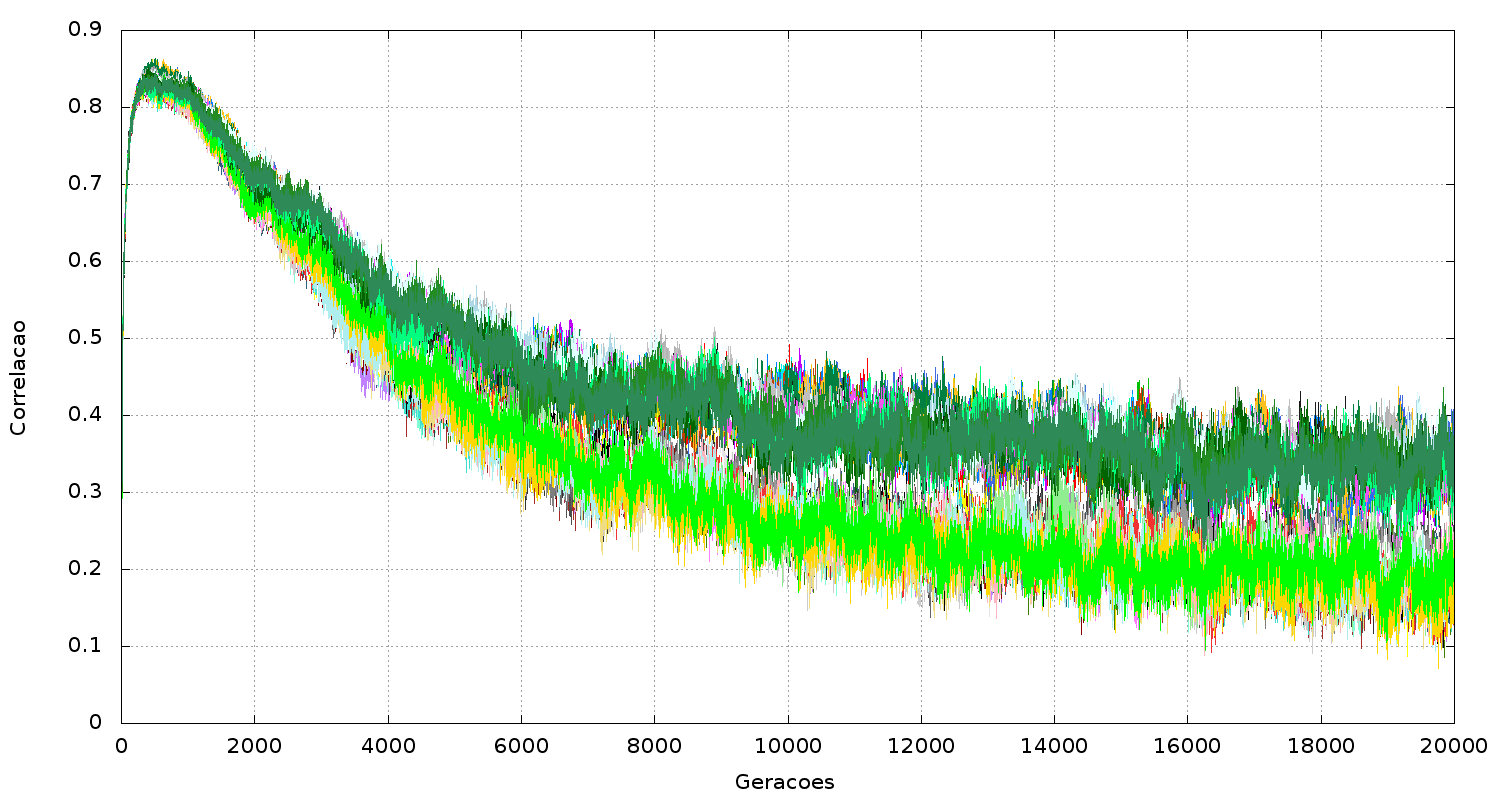
\includegraphics[width=150mm, height=55mm]{figuras/MBLR100.png}}
  \caption{Evolução da correlação entre dez traços ligados por efeitos
  pleiotrópicos controlados por uma função ontogenética linear binária
  variável sofrendo seleção estabilizadora correlacionada e seleção
  direcional intensa para mudança correlacionada dentros dos módulos,
  para diferentes valores do número de alelos. ($Ne=5000$, $\mu/\mu_B=5$, $\Delta_S=0.2$)}
  \label{MBLR}
\end{figure}
\end{center}

\section{Conclusões e Próximos Passos}

Até agora nossos resultados apontam o modelo de matriz $B$ como sendo o
mais adequado aos nossos propósitos de elucidar condições e mecanismos
envolvidos na evolução e manutenção de padrões modulares em populações
naturais. Acreditamos que o uso de alelos mutacionais para representar a
matriz $M$ não seja adequado para simulação de sistemas quantitativos de
muitos traços, por não explorar adequadamente o espaço de fase das
matrizes de correlação dos efeitos mutacionais. A restrição da matriz
ser positiva definida e com valores entre -1 e 1 dificulta a criação de
método de simulação eficiente que possa ser associado a indivíduos,
herdável e ainda possua variação adequada para responder a seleção
imposta. Já a matriz $B$, talvez por sua simplicidade maior no que se
refere a suas mutações e padrão de herança, é capaz de responder
adequadamente à seleção e reproduzir padrões naturais.

Além disso, papéis fundamentais são atribuidos a seleção,
tanto estabilizadora quanto direcional, ambas atuando no surgimento e
manutenção de módulos variacionais. Apesar de explicações nulas terem
sido propostas para o surgimento de módulos em diversos níveis
organizacionais \citep{Lynch2007, Wagner2007}, nossos resultados sugerem
que efeitos seletivos, possivelmente advindos de seleção interna ou
restrições ontogenéticas (aqui representadas pela matriz de seleção
$\omega$), são responsáveis pela evolução de estruturas modulares, pelo
menos no contexto de traços quantitativos e modularidade variacional. 

Essa visão vai de encontro com resultados recentes de trabalhos
computacionais em sistemas morfológicos mais simples
\citep{Pavlicev2010}, e além de simulações focadas em sistemas não
quantitativos \citep{Ancel2000,Espinosa-Soto2010}. A importância de
seleção na manutenção de padrões de covariação também havia sido
sugerida por diversos autores \citep{Cheverud1984, Marroig2001,Porto2008},
e nossos resultados reforçam essa idéia advinda de trabalhos em sistemas
naturais.

Algumas perguntas permanecem sub-exploradas, principalmente devido a
limitações computacionais. O aumento do número de alelos envolvidos na
determinação de cada traços, por exemplo, é extremamente custoso e
difícil de ser explorado quantitativamente. O tamanho populacional já
teve sua importância demonstrada, tanto nos nossos resultados quanto em
\cite{Jones2003} e em diversos outros contextos. Seu aumento é também
custoso e ainda não foi apropriadamente explorado. Além disso, nosso
trabalho até o momento tem caráter qualitativo. Para a
produção de estatísticas quantitativas todas as simulações deverão ser
replicadas, afim de produzir um conjunto de dados de qualidade
quantitativa apropriada.  Esperamos amenizar essas dificuldades num
futuro próximo com o uso de um servidor de processamento dedicado, em
processo de compra pelo nosso laboratório.

\section{Monitoria PAE}

No periodo em questão o aluno realisou uma monitora PAE, atuando como
auxiliar na disciplina Processos Evolutivos, oferecida pelo departamento
de Genética e Biologia Evolutiva. Foram realizados atividades de
preparação e aplicação de listas de exercícios, plantões de dúvidas,
correção de provas e listas alem de controles de presença e notas.

O aluno recebeu uma bolsa CAPES pelo programa PAE por essas
atividades.

\section{Artigos Publicados}

No periodo em questão foi publicado um artigo em revista. Em colaboração
com outros membros do Laborátorio de Evolução de Mamíferos foi produzido
o manuscrito {\it Noise, Modularity and Natural Selection}, publicado na
revista {\it Evolution} \citep{Marroig2011b}.  Segue o
resumo:

\flushright{\it Most biological systems are formed by component parts
that to some degree are inter-related. Groups of parts that are more
associated among themselves and are relatively autonomous from others
are called modules. One of the consequences of modularity is that
biological systems usually present an unequal distribution of the
genetic variation among variables. Estimating the covariance matrix that
describes these systems is a difficult problem due to a number of
factors such as poor sample sizes and measurement errors. We show that
this problem will be exacerbated whenever matrix inversion is required,
as in directional selection reconstruction analysis. We explore the
consequences of varying degrees of modularity and signal-to-noise ratio
on selection reconstruction. We then present and test the efficiency of
available methods for controlling noise in matrix estimates. In our
simulations, controlling matrices for noise vastly improves the
reconstruction of selection gradients. We also perform an analysis of
selection gradients reconstruction over a New World Monkeys skull
database in order to illustrate the impact of noise on such analyses.
Noise-controlled estimates render far more plausible interpretations
that are in full agreement with previous results.}.
\flushleft{}

O artigo pode ser encontrado na integra no sitio \url{http://arxiv.org/abs/1112.1391}.

\section{Reserva Técnica}

Não houveram gastos com reserva técnica no período em questão.

% --- BIBLIOGRAFIA ---

\bibliography{Mestrado}
%\section{Anexos}
%\begin{center}
%\begin{figure}[H]
%  \includegraphics[width= 150mm, height=180mm]{figuras/NFe-578843}
%\end{figure}
%\begin{figure}[H]
%  \includegraphics[width= 150mm, height=180mm]{figuras/CCNFe-578843}
%\end{figure}
%\begin{figure}[H]
%  \includegraphics[width= 150mm, height=180mm]{figuras/NFe-564111}
%\end{figure}
%\begin{figure}[H]
%  \includegraphics[width= 150mm, height=180mm]{figuras/CCNFe-564111}
%\end{figure}
%\begin{figure}[H]
%  \includegraphics[width= 150mm, height=180mm]{figuras/NF-windows}
%\end{figure}
%\end{center}

\end{document}
